% -*- mode:latex; mode:flyspell -*-
\documentclass[10pt, conference, compsocconf]{IEEEtran}


% *** GRAPHICS RELATED PACKAGES ***
%
\ifCLASSINFOpdf
  \usepackage[pdftex]{graphicx}
  \usepackage{color}
  \usepackage{epstopdf}
  %\usepackage[update]{eps2pdf}
  %\usepackage[pdf]{pstricks}
  % declare the path(s) where your graphic files are
  % \graphicspath{{../pdf/}{../jpeg/}}
  % and their extensions so you won't have to specify these with
  % every instance of \includegraphics
  % \DeclareGraphicsExtensions{.pdf,.jpeg,.png}
\else
  % or other class option (dvipsone, dvipdf, if not using dvips). graphicx
  % will default to the driver specified in the system graphics.cfg if no
  % driver is specified.
  % \usepackage[dvips]{graphicx}
  % declare the path(s) where your graphic files are
  % \graphicspath{{../eps/}}
  % and their extensions so you won't have to specify these with
  % every instance of \includegraphics
  % \DeclareGraphicsExtensions{.eps}
\fi




% *** MATH PACKAGES ***
%
%\usepackage[cmex10]{amsmath}
% A popular package from the American Mathematical Society that provides
% many useful and powerful commands for dealing with mathematics. If using
% it, be sure to load this package with the cmex10 option to ensure that
% only type 1 fonts will utilized at all point sizes. Without this option,
% it is possible that some math symbols, particularly those within
% footnotes, will be rendered in bitmap form which will result in a
% document that can not be IEEE Xplore compliant!
%
% Also, note that the amsmath package sets \interdisplaylinepenalty to 10000
% thus preventing page breaks from occurring within multiline equations. Use:
%\interdisplaylinepenalty=2500
% after loading amsmath to restore such page breaks as IEEEtran.cls normally
% does. amsmath.sty is already installed on most LaTeX systems. The latest
% version and documentation can be obtained at:
% http://www.ctan.org/tex-archive/macros/latex/required/amslatex/math/





% *** SPECIALIZED LIST PACKAGES ***
%
%\usepackage{algorithmic}
% algorithmic.sty was written by Peter Williams and Rogerio Brito.
% This package provides an algorithmic environment fo describing algorithms.
% You can use the algorithmic environment in-text or within a figure
% environment to provide for a floating algorithm. Do NOT use the algorithm
% floating environment provided by algorithm.sty (by the same authors) or
% algorithm2e.sty (by Christophe Fiorio) as IEEE does not use dedicated
% algorithm float types and packages that provide these will not provide
% correct IEEE style captions. The latest version and documentation of
% algorithmic.sty can be obtained at:
% http://www.ctan.org/tex-archive/macros/latex/contrib/algorithms/
% There is also a support site at:
% http://algorithms.berlios.de/index.html
% Also of interest may be the (relatively newer and more customizable)
% algorithmicx.sty package by Szasz Janos:
% http://www.ctan.org/tex-archive/macros/latex/contrib/algorithmicx/




% *** ALIGNMENT PACKAGES ***
%
%\usepackage{array}
% Frank Mittelbach's and David Carlisle's array.sty patches and improves
% the standard LaTeX2e array and tabular environments to provide better
% appearance and additional user controls. As the default LaTeX2e table
% generation code is lacking to the point of almost being broken with
% respect to the quality of the end results, all users are strongly
% advised to use an enhanced (at the very least that provided by array.sty)
% set of table tools. array.sty is already installed on most systems. The
% latest version and documentation can be obtained at:
% http://www.ctan.org/tex-archive/macros/latex/required/tools/


%\usepackage{mdwmath}
%\usepackage{mdwtab}
% Also highly recommended is Mark Wooding's extremely powerful MDW tools,
% especially mdwmath.sty and mdwtab.sty which are used to format equations
% and tables, respectively. The MDWtools set is already installed on most
% LaTeX systems. The lastest version and documentation is available at:
% http://www.ctan.org/tex-archive/macros/latex/contrib/mdwtools/


% IEEEtran contains the IEEEeqnarray family of commands that can be used to
% generate multiline equations as well as matrices, tables, etc., of high
% quality.


%\usepackage{eqparbox}
% Also of notable interest is Scott Pakin's eqparbox package for creating
% (automatically sized) equal width boxes - aka "natural width parboxes".
% Available at:
% http://www.ctan.org/tex-archive/macros/latex/contrib/eqparbox/





% *** SUBFIGURE PACKAGES ***
%\usepackage[tight,footnotesize]{subfigure}
% subfigure.sty was written by Steven Douglas Cochran. This package makes it
% easy to put subfigures in your figures. e.g., "Figure 1a and 1b". For IEEE
% work, it is a good idea to load it with the tight package option to reduce
% the amount of white space around the subfigures. subfigure.sty is already
% installed on most LaTeX systems. The latest version and documentation can
% be obtained at:
% http://www.ctan.org/tex-archive/obsolete/macros/latex/contrib/subfigure/
% subfigure.sty has been superceeded by subfig.sty.



%\usepackage[caption=false]{caption}
%\usepackage[font=footnotesize]{subfig}
% subfig.sty, also written by Steven Douglas Cochran, is the modern
% replacement for subfigure.sty. However, subfig.sty requires and
% automatically loads Axel Sommerfeldt's caption.sty which will override
% IEEEtran.cls handling of captions and this will result in nonIEEE style
% figure/table captions. To prevent this problem, be sure and preload
% caption.sty with its "caption=false" package option. This is will preserve
% IEEEtran.cls handing of captions. Version 1.3 (2005/06/28) and later
% (recommended due to many improvements over 1.2) of subfig.sty supports
% the caption=false option directly:
%\usepackage[caption=false,font=footnotesize]{subfig}
%
% The latest version and documentation can be obtained at:
% http://www.ctan.org/tex-archive/macros/latex/contrib/subfig/
% The latest version and documentation of caption.sty can be obtained at:
% http://www.ctan.org/tex-archive/macros/latex/contrib/caption/




% *** FLOAT PACKAGES ***
%
%\usepackage{fixltx2e}
% fixltx2e, the successor to the earlier fix2col.sty, was written by
% Frank Mittelbach and David Carlisle. This package corrects a few problems
% in the LaTeX2e kernel, the most notable of which is that in current
% LaTeX2e releases, the ordering of single and double column floats is not
% guaranteed to be preserved. Thus, an unpatched LaTeX2e can allow a
% single column figure to be placed prior to an earlier double column
% figure. The latest version and documentation can be found at:
% http://www.ctan.org/tex-archive/macros/latex/base/



%\usepackage{stfloats}
% stfloats.sty was written by Sigitas Tolusis. This package gives LaTeX2e
% the ability to do double column floats at the bottom of the page as well
% as the top. (e.g., "\begin{figure*}[!b]" is not normally possible in
% LaTeX2e). It also provides a command:
%\fnbelowfloat
% to enable the placement of footnotes below bottom floats (the standard
% LaTeX2e kernel puts them above bottom floats). This is an invasive package
% which rewrites many portions of the LaTeX2e float routines. It may not work
% with other packages that modify the LaTeX2e float routines. The latest
% version and documentation can be obtained at:
% http://www.ctan.org/tex-archive/macros/latex/contrib/sttools/
% Documentation is contained in the stfloats.sty comments as well as in the
% presfull.pdf file. Do not use the stfloats baselinefloat ability as IEEE
% does not allow \baselineskip to stretch. Authors submitting work to the
% IEEE should note that IEEE rarely uses double column equations and
% that authors should try to avoid such use. Do not be tempted to use the
% cuted.sty or midfloat.sty packages (also by Sigitas Tolusis) as IEEE does
% not format its papers in such ways.





% *** PDF, URL AND HYPERLINK PACKAGES ***
%
%\usepackage{url}
% url.sty was written by Donald Arseneau. It provides better support for
% handling and breaking URLs. url.sty is already installed on most LaTeX
% systems. The latest version can be obtained at:
% http://www.ctan.org/tex-archive/macros/latex/contrib/misc/
% Read the url.sty source comments for usage information. Basically,
% \url{my_url_here}.





% *** Do not adjust lengths that control margins, column widths, etc. ***
% *** Do not use packages that alter fonts (such as pslatex).         ***
% There should be no need to do such things with IEEEtran.cls V1.6 and later.
% (Unless specifically asked to do so by the journal or conference you plan
% to submit to, of course. )


% correct bad hyphenation here
% \hyphenation{op-tical net-works semi-conduc-tor}


\begin{document}
%
% paper title
% can use linebreaks \\ within to get better formatting as desired
\title{A framework for design space exploration for HPC architectures}


% author names and affiliations
% use a multiple column layout for up to two different
% affiliations

\author{\IEEEauthorblockN{Authors Name/s per 1st Affiliation (Author)}
\IEEEauthorblockA{line 1 (of Affiliation): dept. name of organization\\
line 2: name of organization, acronyms acceptable\\
line 3: City, Country\\
line 4: Email: name@xyz.com}
\and
\IEEEauthorblockN{Authors Name/s per 2nd Affiliation (Author)}
\IEEEauthorblockA{line 1 (of Affiliation): dept. name of organization\\
line 2: name of organization, acronyms acceptable\\
line 3: City, Country\\
line 4: Email: name@xyz.com}
}

% conference papers do not typically use \thanks and this command
% is locked out in conference mode. If really needed, such as for
% the acknowledgment of grants, issue a \IEEEoverridecommandlockouts
% after \documentclass

% for over three affiliations, or if they all won't fit within the width
% of the page, use this alternative format:
%
%\author{\IEEEauthorblockN{Michael Shell\IEEEauthorrefmark{1},
%Homer Simpson\IEEEauthorrefmark{2},
%James Kirk\IEEEauthorrefmark{3},
%Montgomery Scott\IEEEauthorrefmark{3} and
%Eldon Tyrell\IEEEauthorrefmark{4}}
%\IEEEauthorblockA{\IEEEauthorrefmark{1}School of Electrical and Computer Engineering\\
%Georgia Institute of Technology,
%Atlanta, Georgia 30332--0250\\ Email: see http://www.michaelshell.org/contact.html}
%\IEEEauthorblockA{\IEEEauthorrefmark{2}Twentieth Century Fox, Springfield, USA\\
%Email: homer@thesimpsons.com}
%\IEEEauthorblockA{\IEEEauthorrefmark{3}Starfleet Academy, San Francisco, California 96678-2391\\
%Telephone: (800) 555--1212, Fax: (888) 555--1212}
%\IEEEauthorblockA{\IEEEauthorrefmark{4}Tyrell Inc., 123 Replicant Street, Los Angeles, California 90210--4321}}




% use for special paper notices
%\IEEEspecialpapernotice{(Invited Paper)}




% make the title area
\maketitle


\begin{abstract}

  In this article we provide a framework for exploiting parallelism onto
  heterogeneous HPC architectures. Given a HPC cluster with varying
  compute units, communication constraints and topology, our framework
  can be utilized for partitioning applications exhibiting task and data
  parallelism resulting in increased throughput. Our framework can also
  be used by designers at an early design stage to explore the type of
  compute units needed and the topology that would be suited for a given
  application, thereby reducing costs and power requirements. Moreover,
  software programmers and compiler writers can utilize our framework to
  gauge the potential parallelism in their programs. The challenge lies
  in the fact that heterogeneous compute clusters consist of processing
  elements exhibiting different compute speeds, vector lengths, and
  communication bandwidths, which all need to be considered when
  partitioning the application and associated data. We tackle this
  problem using a staged graph partitioning framework. Our experiments
  show an order of magnitude speedup for applications. Furthermore our
  framework finishes within seconds even when simulating 100's of
  processing elements, which makes our architecture suitable for
  exploring parallelism potential at compile time.

  % In this paper we solve the problem of partitioning applications with a
  % mixture of both: task-parallel and data-parallel parts onto
  % heterogeneous compute clusters. The challenge lies in the utilization
  % of vector and non-vector processing elements, while accounting for
  % varying communication latencies and bandwidths. We propose a graph
  % partitioning heuristic, which clusters a heterogeneous topology into a
  % homogeneous one and then partitions the applications onto the
  % resultant cluster in stages. Our experiments show that our approach is
  % results in X\% better application run-times, while being fast making
  % it suitable as a compilation time technique.

\end{abstract}

\begin{IEEEkeywords}
  Graph partitioning, vectorization, data parallelism, heterogeneous
  architectures, clusters.
\end{IEEEkeywords}


% For peer review papers, you can put extra information on the cover
% page as needed:
% \ifCLASSOPTIONpeerreview
% \begin{center} \bfseries EDICS Category: 3-BBND \end{center}
% \fi
%
% For peerreview papers, this IEEEtran command inserts a page break and
% creates the second title. It will be ignored for other modes.
\IEEEpeerreviewmaketitle

\section{Introduction}
\label{sec:introduction}

High Performance Computing (HPC) clusters increasingly consist of large numbers
of heterogeneous
processing elements such as CPUs, graphics processing units (GPUs),
field programmable gate arrays (FPGAs), low-power processors intended
for digital signal processing (DSP), etc. By combining heterogeneous
processing units it may be possible to divide the work so that different
types of computation in the application are run on different types of
units. This can result in significant speed-ups, lower hardware costs
and/or reduced power consumption by the HPC system.  For example, if a
computation contains the right patterns of data parallelism it may run
dozens or even hundreds of times faster on a GPU than on a CPU that has
similar cost and power consumption. On the other hand, computations with
less data parallelism and more complex control flow may run faster on
CPUs. Matching the type of computation to the processor can yield
significant benefits.

Although the potential of heterogeneous computing is great, exploiting
that potential is more difficult. Given a parallel application, it is
difficult to map the available parallelism onto the hardware. For
example, how does one decide which parallel filters should run on which
type of execution unit? Given a system with dozens or hundreds of CPUs,
GPUs and other units, how does one divide the work between them?  There
are several conflicting factors. For example, one wants to allocate
filters to the type of execution unit that will execute it most
efficiently. On the other hand, one wants to achieve a good load balance
by dividing the work evenly across the units. % At the same time, one must
% respect data dependencies between filters. And finally, data
% communication costs between processing elements can be substantial,
% and are usually themselves heterogeneous. Communication with nearby
% processing elements is usually much faster than communication with
% more distant ones.
We want to allocate the filters to reduce communication costs while at the
same time taking account of all the other factors.

In this paper we consider the problem of mapping graphs of parallel
tasks to heterogeneous HPC computing systems. This problem has been
studied extensively for homogeneous architectures where all processing
elements are the same. Although the homogeneous case is
NP-hard~\cite{vsar89}, several heuristic solutions have been found that
work well in practice. However, extending these solutions to the
heterogeneous case is difficult for two reasons.

% Firstly, good solutions to the homogeneous case often work well by
% dividing the filters evenly across the available processors. However,
In the heterogeneous case some processing elements are more powerful
than others, so achieving a good load balance usually involves
distributing the work unevenly. % So we need algorithms the will divide
% the work between processing elements according to their processing
% capability.

A second reason why it can be difficult to extend algorithms for
homogeneous architectures to the heterogeneous hardware relates to the
strengths and weaknesses of different types of processors. When
considering heterogeneous architectures, it is tempting to think of
some processing elements simply being more powerful than others. % For
% example, we might think of a system with 64 processors capable of X
% performance, and 16 processors capable of 2X performance. Such
% machines exist. But many heterogeneous HPC machines contain different
% \textit{types} of processing elements, such as CPUs and GPUs.
A GPU is not simply a more powerful CPU. In fact, some types of
computation run better on CPUs and some on GPUs.  For a mapping
algorithm to work well, it needs to take account of the strengths and
weaknesses of different types of processing elements. In this paper we
present an approach to mapping parallel tasks to heterogeneous
architectures that addresses both of these concerns.

Our \textbf{main contributions} are as follows:
\begin{itemize}
\item We present a novel approach to characterizing the type of
  processing elements based on their level of vector parallelism which
  allows us to distinguish the suitability of different types of units
  to different filters.
\item We provide a novel algorithm for mapping task and data parallelism
  to heterogeneous architectures based on hierarchical graph
  partitioning.
%\item In addition to mapping filters to processing elements, our framework
%  also allocates the data stores being used by the different filters.
% \item We provide an experimental evaluation of these techniques
% and compare with other algorithms.
\end{itemize}

The rest of this paper is organized as follows.
Section~\ref{sec:preliminaries} formalizes the problem statement and
defines the objective function. Next, in
Section~\ref{sec:our-framework}, we provide a detailed description of
our framework. % In Section~\ref{sec:imple} we
% then describe the implementation of our approach.
Section~\ref{sec:experiments-results} gives the quantitative
comparisons of our approach against other
approaches. Section~\ref{sec:related-work} describes the related work
and positions our approach in comparison to these works.  Finally, we
conclude in Section~\ref{sec:conclusion}.

% \section{Motivating Example}
% \label{sec:motivating-example}
% Consider the code snippet in Figure~\ref{fig:2} that carries out the
% main stencil computation using the Jacobi algorithm. Jacobi is used
% for solving large systems of linear equations, especially for heat
% transfer problems and numerical fluid mechanics. We have chosen this
% as our motivating example because it has been successfully
% parallelized using MPI~\cite{jacobi1} and CUDA~\cite{jacobi2}.  There
% is a great deal of potential to use both techniques together to gain
% further speed-up. The CUDA programming techniques exploit the
% \textit{Single Instruction Multiple Data} (SIMD) potential in the
% Jacobi algorithm~\cite{jacobi2} by modelling parallelism as vector
% computations suitable for a GPU. The MPI approach on the other hand
% exploits \textit{Multiple Instruction Multiple Data} (MIMD) potential
% by distributing the parallelism across different CPU nodes. To
% maximize speed-up we would like to exploit both SIMD and MIMD
% parallelism in heterogeneous architectures.

% % One way to represent program parallelism is to build a filter graph.  A
% % filter graph is a graph where the nodes represent computation and the
% % edges represent data dependencies between the computations.
% Figure~\ref{fig:1} shows a simple filter graph for the Jacobi code. There
% are many ways in which the filter graph can be built. In the current
% paper, the filter graph is built using a parallelizing compiler that
% % <<<<<<< HEAD
% automatically detects filter parallelism in code that operates on
% arrays. Each node in the graph corresponds to one of the assignment
% % ======= automatically detects simple data parallelism in code that
% % operates on arrays.  Each node in the graph corresponds to one of the
% % assignment >>>>>>> 42ffdc746763a12ade4dfcf6d9c9091b66029af3
% statements in the Jacobi source code in Figure~\ref{fig:2}.

% % Note that although each node in our version of the filter graph contains
% % just a single assignment statement,
% Each of those statements is executed many times, and in fact there is a
% great deal of data parallelism in each node. This data parallelism can
% be exploited using either SIMD parallelism (found in CPUs with vector
% units and GPUs) or MIMD parallelism (by using multiple processing
% elements to perform the computation) or a combination of both. % Thus, to
% % map the filter graph to a heterogeneous architecture we need to be aware
% % both of the number and type of available processing elements and the
% % amount of available SIMD parallelism available within each type of
% % processing element.
% Therefore, we annotate the filter graph with the amount of SIMD
% parallelism available in each node, as described in
% Section~\ref{sec:preliminaries}.

% % By annotating the filter graph nodes with the level of available SIMD
% % parallelism it is possible to make better mapping decisions.  For
% % example, GPUs typically offer very high levels of SIMD parallelism but
% % perform poorly on code with little data parallelism.

% % In addition to allocating these filters based on appropriate levels of SIMD
% % parallelism, it is also important to divide the overall work of the
% % filter graph across the available resources.

% Heuristics developed for homogeneous architectures that divide the work
% evenly among the resources do not work well for heterogeneous
% architectures. This is because one might execute sequential code very
% efficiently while another provides a lot of SIMD parallelism making it a
% challenge to divide the filters. Moreover, this causes the communication
% volume between resources to be very different. In such a case any
% imbalance in communication could severely impact the performance of the
% application, making it important to account for the communication costs
% between the resources when mapping the filter graph.

% \begin{scriptsize}
%   \begin{figure}[h!]
%     \centering
%     \caption{}
%     \label{fig:2}
%   \end{figure}
% \end{scriptsize}

% Our solution to this problem is to hierarchically partition the nodes
% present in the heterogeneous architecture into clusters as described in
% section~\ref{sec:clustering-topology}. The clusters are created such that
% the computation capacity is balanced across clusters and the
% communication volume between them are minimized. An example of such
% recursive clustering is shown in Figure \ref{fig:res}. Once the machine
% has been divided into a hierarchy of clusters, we partition the filter
% graph across the clusters until we reach the lowest level where each
% filter is allocated to a specific resource as described in
% section~\ref{sec:filter-graph-part}.

%~ David's Text
%~ In addition to allocating filters to PEs with appropriate levels of SIMD
%~ parallelism, it is also important to divide the overall work of the
%~ filter graph across the available PEs. However, there are two
%~ major problems with doing this for a heterogeneous target architecture.
%~ First, the capabilities of the different PEs may be very different.
%~ One might execute sequential code very efficiently while another
%~ provides a lot of SIMD parallelism. Heuristics developed for
%~ homogeneous architectures that divide the work evenly among the PEs do
%~ not work well for heterogeneous architectures. Seconldly, we must take
%~ account of communication costs between PEs.
%~
%~ Our solution to this problem is to hierarchically partition the
%~ processing elements into clusters, as shown in Figure \ref{fig:res}.
%~ We partition the available PEs so that each cluster has approximately
%~ the same level of computing capacity, and so that there is plenty of
%~ communication capacity within clusters. We start a cluster consisting
%~ of all PEs in the machine, and this full machine is divided into
%~ (usually) two clusters of approximately equal processing capacity.
%~ The resulting clusters are divided recusively into sub-clusters with
%~ approximately equal capacity.
%~
%~ Once the machine has been divided into a hierarchy of clusters,
%~ we partition the filter graph across the clusters. At each level
%~ of the hierarchy of clusters, the capacity of each cluster has
%~ approximately equal computational capacity. Therefore, simple
%~ graph partitioning algorithms aimed at an even split of the
%~ graph work well. At each level of the hierarchy of clusters
%~ we divide the filter graph among the clusters, until we reach the
%~ lowest level where each filter is allocated to a specific processing
%~ element.


% \section{Introduction and motivating example}
% \label{sec:intr-motiv-example}

% Today's HPC clusters consists of a large number of heterogeneous
% processing elements such as CPUs, GPUs, DSPs, FPGAs, etc. Given an
% application, how does one determine if there are portions of the
% application that should be mapped to a GPU, others to a CPU, and still
% others to an FPGA, and so on? Further, given a heterogenous collection
% of GPUs (i.e., different GPUs may have different vector lengths) and a
% heteorogeneous collection of CPUs (i.e., different CPUs may have
% different number of cores), how do you further decide which portions of
% the GPU should be allocated to a given GPU and not to another GPU? Now
% let us add the final complexity: how do you do the above allocation
% automatically? How do you automatically map the parallelism available in
% an application to the right computation engine from among a
% heterogeneous suite of engines?  This paper offers one such
% approach. What if you do not have the architecture figured out yet but
% you have the application? In this case, one can use our approach to
% determine the type of architecture best suited to map the parallelism
% available in a given application.  Our proposed framework can be used by
% topology designers to quickly carry out a design space exploration to
% determine the type of underlying topology best suited for a given
% application.  Moreover, compiler writers can also use our framework when
% vectorizing and partitioning large vector units onto parallel GPU/CPU
% units.
% % \textbf{AVINASH - PLS CHECK
% % THE LAST CLAIM. DO YOU DO THAT IN THIS PAPER?}

% Consider the code snippet in Figure~\ref{fig:2} that carries out the
% main stencil computation using the Jacobi algorithm. Jacobi is an
% important stencil computation, which is used for solving large systems
% of linear equations, especially for heat transfer problems and numerical
% fluid mechanics. We have chosen this as our motivating example because
% there have been attempts to parallelize Jacobi using MPI~\cite{jacobi1}
% and CUDA~\cite{jacobi2} with success, making it an important problem to
% solve on a heterogeneous compute cluster mixing MPI and CUDA programming
% techniques and with the potential of making it faster still. The CUDA
% programming techniques exploit the \textit{Single Instruction Multiple
%   Data} (SIMD) potential in the Jacobi algorithm~\cite{jacobi2} by
% modeling parallelism as vector computations suitable for a GPU. The MPI
% approach on the other hand exploits \textit{Multiple Instruction
%   Multiple Data} (MIMD) potential by modeling the parallelism across
% different CPU nodes. Both techniques result in 3-4 times speedup
% compared to single CPU implementations. The challenge when
% \textit{re-designing} and \textit{tuning} such parallel applications to
% exploit vector units \textit{or} MPI alone is well
% documented~\cite{jacobi1,jacobi2}. The complexity of re-designing for a
% mixture of two grows exponentially. The growth in complexity of design
% space is due to a number of factors, some of which we enumerate below:


% \begin{scriptsize}
%   \begin{figure}[h!]
%     \centering
% \begin{verbatim}
%  //Task and data-parallel
%  for (int i=0;i<M; ++i){
%   for (int j=0;j<N; ++j){
%    1: A[i][j] = (i*j+2.0+2.0/N)
%    2: B[i][j] = (i*j+3.0+3.0/N)
%   }
%  }
%  for (int k=0;k<TSTEPS;++k){
%   for (int i=1; i<M; ++i)
%    for (int j=1; j<N; ++j)
%     3: B[i][j] = 0.2*(A[i][j]+A[i][j-1]
%               +A[i][j+1]+A[i-1][j])

%   //Data-parallel
%   for (int i=1; i<M; ++i)
%    for (int j=1; j<N; ++j)
%     4: A[i][j] = B[i][j]
%  }
% \end{verbatim}
%     \caption{Example 2-dimensional Jacobi application}
%     \label{fig:2}
%   \end{figure}
% \end{scriptsize}



% \begin{itemize}

% \item The vector lengths of the underlying processing elements
%   differ. Intel processors have 256 bit vector instructions, while the
%   GPU range varies.

%   % For example, a GPU warp (the smallest vector size) varies from 16-32
%   % scalar instructions. Moreover, these warps can be arranged in
%   % different block sizes, which results in different effective vector
%   % lengths. On the CPU the vector lengths differ themselves, but the
%   % variation is much smaller. For example, the new Intel AVX units have
%   % a
%   % vector length of 256 bits, while the SSE units have a vector length
%   % of
%   % 128 bits.

% \item The actual data-type results in different utilization of vector
%   units. For example, a \texttt{double} type requires twice as many
%   vector registers to carry out processing as compared to an
%   \texttt{int} type.

% \item The size of the vector length and the number of vector units
%   required needs to be determined: simply dividing the data-parallel
%   vector units onto the largest available vector processing elements
%   does not necessarily result in good application throughput or
%   latency. In an ideal scenario for very large vector computations, the
%   vector units can be utilized completely and the rest of the
%   data-parallelism can be exploited in parallel on a CPU unit
%   iteratively in a loop.

% \item The bottleneck of the communication fabric plays an important role
%   in the partitioning problem. Note that in a heterogeneous compute
%   cluster the communication latencies and bandwidths themselves vary.

% \item Allocation of data-stores being utilized by the different
%   processing elements needs to be handled.

% \item Applications written in different ways result in different
%   parallelism potential.

% \item Finally, the scheduling problem is known to be
%   NP-hard~\cite{vsar89}. Thus, we need a good heuristic solution, which
%   finishes quickly and gives good results.

% \end{itemize}

% There are a number of other applications where parallelism plays an
% important
% role. % (\textbf{THIS STATEMENT IS TOO OBVIOUS TO BE MADE A POINT
%   % OF.  UNLESS YOU ARE SAYING THAT THESE APPS HAVE POTENTIAL FOR
%   % EXPLOITING HETEROGENOUS RESOURCES. ARE YOU SAYING THAT?})
% For example, binomial option pricing~\cite{ssol10,hpra10},
% k-means~\cite{jzha11}, Gauss-Seidel stencil computations~\cite{hcou09},
% etc, are well suited to be optimized across heterogeneous HPC
% architectures. Exploiting both data and filter parallelism is essential in
% the general case.

% The rest of the paper is arranged as follows:
% Section~\ref{sec:related-work}, describes the related work and positions
% our approach in comparison to this
% work. Section~\ref{sec:preliminaries}, formalizes the problem
% statement and defined the objective function. Next, in
% Section~\ref{sec:our-framework}, we provide a detailed description of
% our framework. In Section~\ref{sec:imple}, we then describe the
% implementation of our approach. Section~\ref{sec:experiments-results},
% give the quantitative comparisons of our approach against a number of
% other approaches. Finally, we conclude in Section~\ref{sec:conclusion}.

% \section{Introduction and motivating example}
% \label{sec:intr-motiv-example}

% Today's HPC clusters consists of a large number of heterogeneous
% processing elements such as CPUs, GPUs, DSPs, FPGAs, etc. Given an
% application exhibiting potential for parallelism the question remains:
% how does one determine the type of architecture best suited to extract
% this parallelism? Or given an architecture, how does one determine how
% to exploit the potential parallelism in the applications.

% \begin{scriptsize}
%   \begin{figure}[h!]
%     \centering
% \begin{verbatim}
%  //Task and data-parallel
%  for (int i=0;i<M; ++i){
%   for (int j=0;j<N; ++j){
%    1: A[i][j] = ((((i)*((j)+2.0))+2.0)/(N))
%    2: B[i][j] = ((((i)*((j)+3.0))+3.0)/(N))
%   }
%  }
%  for (int k=0;k<TSTEPS;++k){
%   for (int i=1; i<M; ++i)
%    for (int j=1; j<N; ++j)
%     3: B[i][j] = 0.2*(A[i][j]+A[i][j-1]
%               +A[i][j+1]+A[i-1][j])

%   //Data-parallel
%   for (int i=1; i<M; ++i)
%    for (int j=1; j<N; ++j)
%     4: A[i][j] = B[i][j]
%  }
% \end{verbatim}
%     \caption{Example 2-dimensional Jacobi application}
%     \label{fig:2}
%   \end{figure}
% \end{scriptsize}

% Consider the code snippet in Figure~\ref{fig:2} that carries out the
% main stencil computation using the Jacobi algorithm. Jacobi is an
% important stencil computation, which is used for solving large systems
% of linear equations, especially for heat transfer problems and numerical
% fluid mechanics. We have chosen this as our motivating example, because
% there have been attempts to parallelize Jacobi using MPI~\cite{jacobi1}
% and CUDA~\cite{jacobi2} with success, making it an important problem to
% solve on a heterogeneous compute cluster mixing MPI and CUDA programming
% techniques and with the potential of making it faster still. The CUDA
% programming techniques exploit the \textit{Single Instruction Multiple
%   Data} (SIMD) potential in the Jacobi algorithm~\cite{jacobi2} by
% modeling parallelism as vector computations suitable for a GPU. The MPI
% approach on the other hand exploits \textit{Multiple Instruction
%   Multiple Data} (MIMD) potential by modeling the parallelism across
% different CPU nodes. Both techniques result in 3-4 times speedup
% compared to single CPU implementations. The challenge when
% \textit{re-designing} and \textit{tuning} such parallel applications to
% exploit vector units \textit{or} MPI alone is well
% documented~\cite{jacobi1,jacobi2}. The complexity of re-designing for a
% mixture of two grows exponentially. The growth in complexity of design
% space is due to a number of factors, some of which we enumerate below:

% \begin{itemize}

% \item The vector lengths of the underlying processing elements
%   differ. Intel processors have 256 bit vector instructions, while the
%   GPU range varies.

%   % For example, a GPU warp (the smallest vector size) varies from 16-32
%   % scalar instructions. Moreover, these warps can be arranged in
%   % different block sizes, which results in different effective vector
%   % lengths. On the CPU the vector lengths differ themselves, but the
%   % variation is much smaller. For example, the new Intel AVX units have
%   % a
%   % vector length of 256 bits, while the SSE units have a vector length
%   % of
%   % 128 bits.

% \item The actual data-type results in different utilization of vector
%   units. For example, a \texttt{double} type requires twice as many
%   vector registers to carry out processing as compared to an
%   \texttt{int} type.

% \item The size of the vector length and the number of vector units
%   required needs to be determined: simply dividing the data-parallel
%   vector units onto the largest available vector processing elements
%   does not necessarily result in good application throughput or
%   latency. In an ideal scenario for very large vector computations, the
%   vector units can be utilized completely and the rest of the
%   data-parallelism can be exploited in parallel on a CPU unit
%   iteratively in a loop.

% \item The bottleneck of the communication fabric plays an important role
%   in the partitioning problem. Note that in a heterogeneous compute
%   cluster the communication latencies and bandwidths themselves vary.

% \item Allocation of data-stores being utilized by the different
%   processing elements needs to be handled.

% \item Applications written in different ways result in different
%   parallelism potential.

% \item Finally, the scheduling problem is known to be
%   NP-hard~\cite{vsar89}. Thus, we need a good heuristic solution, which
%   finishes quickly and gives good results.

% \end{itemize}

% There are a number of other applications where parallelism plays and
% important role. For example, binomial option pricing, k-means
% calculations, Gauss-Seidel stencil computations, etc, are well suited to
% be optimized across heterogeneous HPC architectures. In general we have
% found it is much more essential to exploit data-parallelism as compared
% to filter-parallelism to achieve speedups. But, exploiting both types of
% parallelism is essential in the general case.

% In this paper we propose a framework, which can be used by topology
% designers, and application writers to quickly carry out a design space
% exploration to determine the type of underlying topology best suited for
% a given application. Moreover, compiler writers can also use our
% framework when vectorizing to partition large vector units onto parallel
% GPU/CPU units.



%%% Local Variables:
%%% mode: latex
%%% TeX-master: "bare_conf"
%%% End:


\section{Related work}
\label{sec:related-work}

A significant amount of research literature exists for extracting
parallelism from programs~\cite{mgri98,jdon06,mgor06,gsih93,pcar09}. The
polyhedral optimization model~\cite{mgri98} concentrates on extracting
parallelism from loops, which is a form of data-parallelism. The
polyhedral optimization community has concentrated on optimizing for
CPUs and GPUs separately, but to our knowledge has not explored the
combination of the two. Carpenter et. al~\cite{pcar09} have again
explored ideas for partitioning onto heterogeneous architectures, but at
a much smaller scale and again ignoring data-allocation costs and
depending upon the polyhedral model for vectorization. The
StreamIt~\cite{wthi02} community has also explored parallelization
techniques, but they have only targeted homogeneous RAW~\cite{ewai97}
architecture. There are the classical algorithms such as critical path
scheduling~\cite{Kohler1975} and list scheduling~\cite{atho74}, which
have been used for scheduling task parallel process onto homogeneous
architectures. The list scheduling techniques targeting heterogeneous
architectures such as~\cite{htop02} do not exploit SIMD parallelism onto
vector processors. Declustering~\cite{gsih93}, is another technique,
which misses the opportunity to mix SIMD and task-parallel optimizations
together.

Cluster based partitioning techniques~\cite{mmah99,adou04,tbra01} only
consider independent tasks without communication. The proposed
heuristics for partitioning data-parallel applications onto
clusters~\cite{ssan05,skum02} do not consider vectorization potential
available on the compute clusters and only concentrate on partitioning
task parallel processes.

Random search techniques use a specific objective and random
choices to guide them through a search space to arrive at a solution. The
objective is usually derived from information obtained from previous random
searches or prior knowledge about the system. Genetic Algorithms
(GA)~\cite{265940,shroff1996genetic,singh1995mapping,wang1996genetic} is a
commonly used algorithm from this technique and generate reasonably good
results. The drawback being this requires significantly more time than
heusristic based algorithms~\cite{tbra01}. Moreover these techniques often give
such good results due to a unique set of parameters. Determining such optimal
parameters to fine tune these random techniques to get good results is a
challenge of its own. Moreover Parameters that give good results for a certain
scenario may not be the same for a different one.

Several other techniques also exist that belong to the same category in
addition to GA such as simulated annealing ~\cite{shroff1996genetic,664363} and
local search methods~\cite{622584,537394} which suffer from the same
disadvantages.



%%% Local Variables:
%%% mode: latex
%%% TeX-master: "bare_conf"
%%% End:


\section{Preliminaries}
\label{sec:preliminaries}

First of all, in this section, we present a formal description of the
problem along with the notations used.

\subsection{Notations}

We refer to our application graph, as a \textit{Static Task Graph} (STG)
defined formally as a weighted directed graph: $G_t(V_t, E_t)$, where
$V_t$ is the set of all tasks in the application graph and $E_t$
represents the communication between these tasks. The system resources
are represented by a weighted undirected graph $G_r(V_r, E_r)$ where
$V_r$ represents a set of processing elements which can have different
processing capabilities. Each vertex in the task graph, $t_i \in V_t$ is
referred to as tasks and each vertex in the resource graph, $r_i \in
V_r$ is referred to as processing elements (PEs). % We use $N_T$ to denote
% the total number of tasks in the task graph and $N_R$ to denote the
% total number of processing elements. By our definition of previous
% notations, it follows that $N_T = |V_t|$ and $N_R = |V_r|$.

\subsection{Problem Definition}

Given a graph $G_t(V_t, E_t)$, each vertex in the task graph, $t_i \in
V_t$ has a set of associated requirements represented by $T^{i}_{j}$
where $j=0...n$ with $n$ being the number of requirements for the task
node. These requirements represent the computational requirement of the
kernel. Consider the task graph in Figure~\ref{fig:1} for the running
Jacobi example. The \texttt{boxed} statements give the number of
instructions and the vector count requirements ($T^i_0\ \mathrm{and}\
T^i_1$). The communication edges ($(t_i, t_j) \in E_t$) between
data-stores (\texttt{boxed} statements without the constraints in
Figure~\ref{fig:1}) and the execution statements represent the amount of
data that needs to be transfered from the store and its utilization at
the statement level. Every communication link is weighted with the
amount of data that has to be transferred denoted by $e^c, \forall E_t
\in (V_t \times V_t)$ The task graphs are generated directly from the
program by our compiler. More information about the generation of the
task graphs is provided later in Section~\ref{sec:build-appl-graph}.

% From the perspective of the running example, constraint 0 of the first
% statement ($3$), represented by $T^{1}_{c0}$ denotes ----Avinash add
% some text here referring to the running jacobi example please----. Each
% edge $(t_i, t_j) \in E_t$ corresponds to the amount of data that has to
% be transferred from task $t_i$ to task $t_j$.

Similarly we have a resource graph $G_r(V_r, E_r)$ where each vertex
denotes a processing element. It consists of a set of vertices $V_r =
\{r_1, r_2, ... , r_n\}$ and a set of edges $E_r$. Each processing
element $r_i \in V_r$ has a set of decorations, that represent the
computational capabilities of the processing elements, represented by
$R^{i}_{j}$ where $j=0...n$ with $n$ being the number of constratins for
the resource node. For some resource graph shown in
Figure~\ref{fig:res}, which has $|V_r|$ nodes and 2 capabilities. For
each node, capability 1 ($R^i_0$) epresents the frequency of the PE or
how many scalar instructions the PE can perform in one second (the
\textit{Million Instructions Per Second} (MIPS) count). Capability 2
($R^i_1$) denotes the maximum number of parallel vector operations it
can perform (the vector length). Each edge $e \in E_r$ has a weight
whcih represents the latency/bandwidth between two PEs $r_i$ and $r_j$
which is denoted by $E^c, \forall E_r \in (V_r \times V_r)$.

% While generating the resource graph, we might have to contract edges(becaus we
% contract nodes). Contracting an edge $e=\{i,j\}$ means to replace vertices $i$ and
% $j$ by a new vertex $k$ such that $R^k_0 = R^i_0 + R^j_0$ and $R^k_1 = R^i_1 +
% R^j_1$. All edges of the form $\{i,x\}$ and $\{j,x\}$ for $x \in V_r$ are replaced
% by $\{k,x\}$. If both edges $\{i,x\}$ and $\{j,x\}$ exist, we form the new edge weight
% as defined by $E^{\{w,x\}} = E^{\{i,x\}} + E^{\{j,x\}}$ More information about the
% generation about the generation of the resource graphs is provided later in
% Section~\ref{sec:gener-reso-graph}.

The problem at hand is to effectively map the said task graph $G_t$ onto
given resource graph $G_r$. This problem is reminiscent of a problem of
bin packing which is known to be NP-Hard~\cite{vsar89}. This immediately
implicates that we have to look for heuristic solutions.

To decide if a mapping is effective enough or not, we need an objective
function that defines how good a mapping of tasks onto resources
is. This is denoted by our cost function. Given some application node $i
\in V_t$ mapped to some resource $j \in V_r$, the latency for that node
is computed as: $((T^i_1/R^j_1\times T^i_0)/R^j_0) + (e^d/E^c) | d =
(i,k), k \neq i, \forall k \in V_t, c = (j,l), l \neq j, \forall l \in
V_r $. In this formulation for some task $i$ being mapped onto some
resource $j$, we first calculate the number of vectorized instructions
that can be executed in parallel (by dividing required vector length by
the vector capacity of $j$ represented by $R^j_1$). We then multiply
this number by the number of iterative (non-vectorized) instructions
required to get the total number of instructions to be performed by that
task-graph node. Once we have this number we calculate latency of
execution of this task-graph node $i$ on this resource $j$ by dividing
it with the MIPS value of the resource denoted by $R^j_0$. Calculation
of the communication latency is rather simple, we divide the number of
bits required to be transferred by the bandwidth of the shortest path.

Given the task-graph and the resource-graph, let $\zeta$ be all possible
mappings of the application on the resource-graph. For a particular
mapping $\mathcal{M}$ defined as $\zeta_\mathcal{M}$ on some resource $s
\in V_r$ the mapping latency is defined as:

\begin{equation}
  \begin{array}{c}
    Latency^{\zeta_\mathcal{M}}_s = comp^{\zeta_\mathcal{M}}_s +
comm^{\zeta_\mathcal{M}}_s\\
	\\comp^{\zeta_\mathcal{M}}_s = 
    \sum_{\forall i \in V_t \wedge
      \zeta_\mathcal{M} = s} ((T^i_1/R^s_1\times T^i_0)/R^c_0)\\
    \\comm^{\zeta_\mathcal{M}}_s =
    \sum_{\forall i \in V_t \wedge
      \zeta_\mathcal{M} = s} e^d / E^c\\ 
    \\s.t., d = (i,k), k \neq i, \forall k
    \in V_t \wedge\  c = (s,l), l \neq s, \forall l \in V_r
  \end{array}
  \label{eq:1}
\end{equation}

Finally, the complete application latency can then be defined as: 
\begin{equation}
  \label{eq:2}
  Latency^{\zeta_\mathcal{M}} = max_{s}
  ({Latency^{\zeta_\mathcal{M}}_s}), \forall s \in V_t
\end{equation}

The objective of our framework is to find a mapping $\zeta_\mathcal{M}$
that minimizes the total application latency as described in
Equation~(\ref{eq:2}).

\subsection{Key Contributions}
Our key contributions in the article are as follows:
\begin{itemize}
\item A novel way for compiler writers and software programmers to gauge
  the potential performance of their programs on any given architecture.
\item A framework that allows topology designers to efficaciously
  explore the design space to determine the type of underlying
  architecture that would suit a given application.
\item A new heuristic based framework that exploits task and data
  parallelism exhibited by applications for mapping them onto
  heterogeneous HPC architectures.
\item Along with mapping application-tasks onto resource nodes, the
  framework also allocates data-stores being utilized by the different
  application-tasks.
\item A rigorous experimental setup to analyse the effectiveness of our
  framework.
\end{itemize}

\section{Our framework}
\label{sec:our-framework}

In this section we describe our heuristic algorithm. There are three
important concepts that need description. First, we describe how we
extract fine grained parallelism from the application into the task
graph. Next, we describe how the topology clusters are formed from the
resource graphs accounting for communication and heterogeneity of the
topology. Finally, we describe how the mapping is performed.

% -*- mode:latex; mode:flyspell -*-
\subsection{Generating the task graph}
\label{sec:build-appl-graph}

\begin{figure*}[t!]
  % \centering
  % 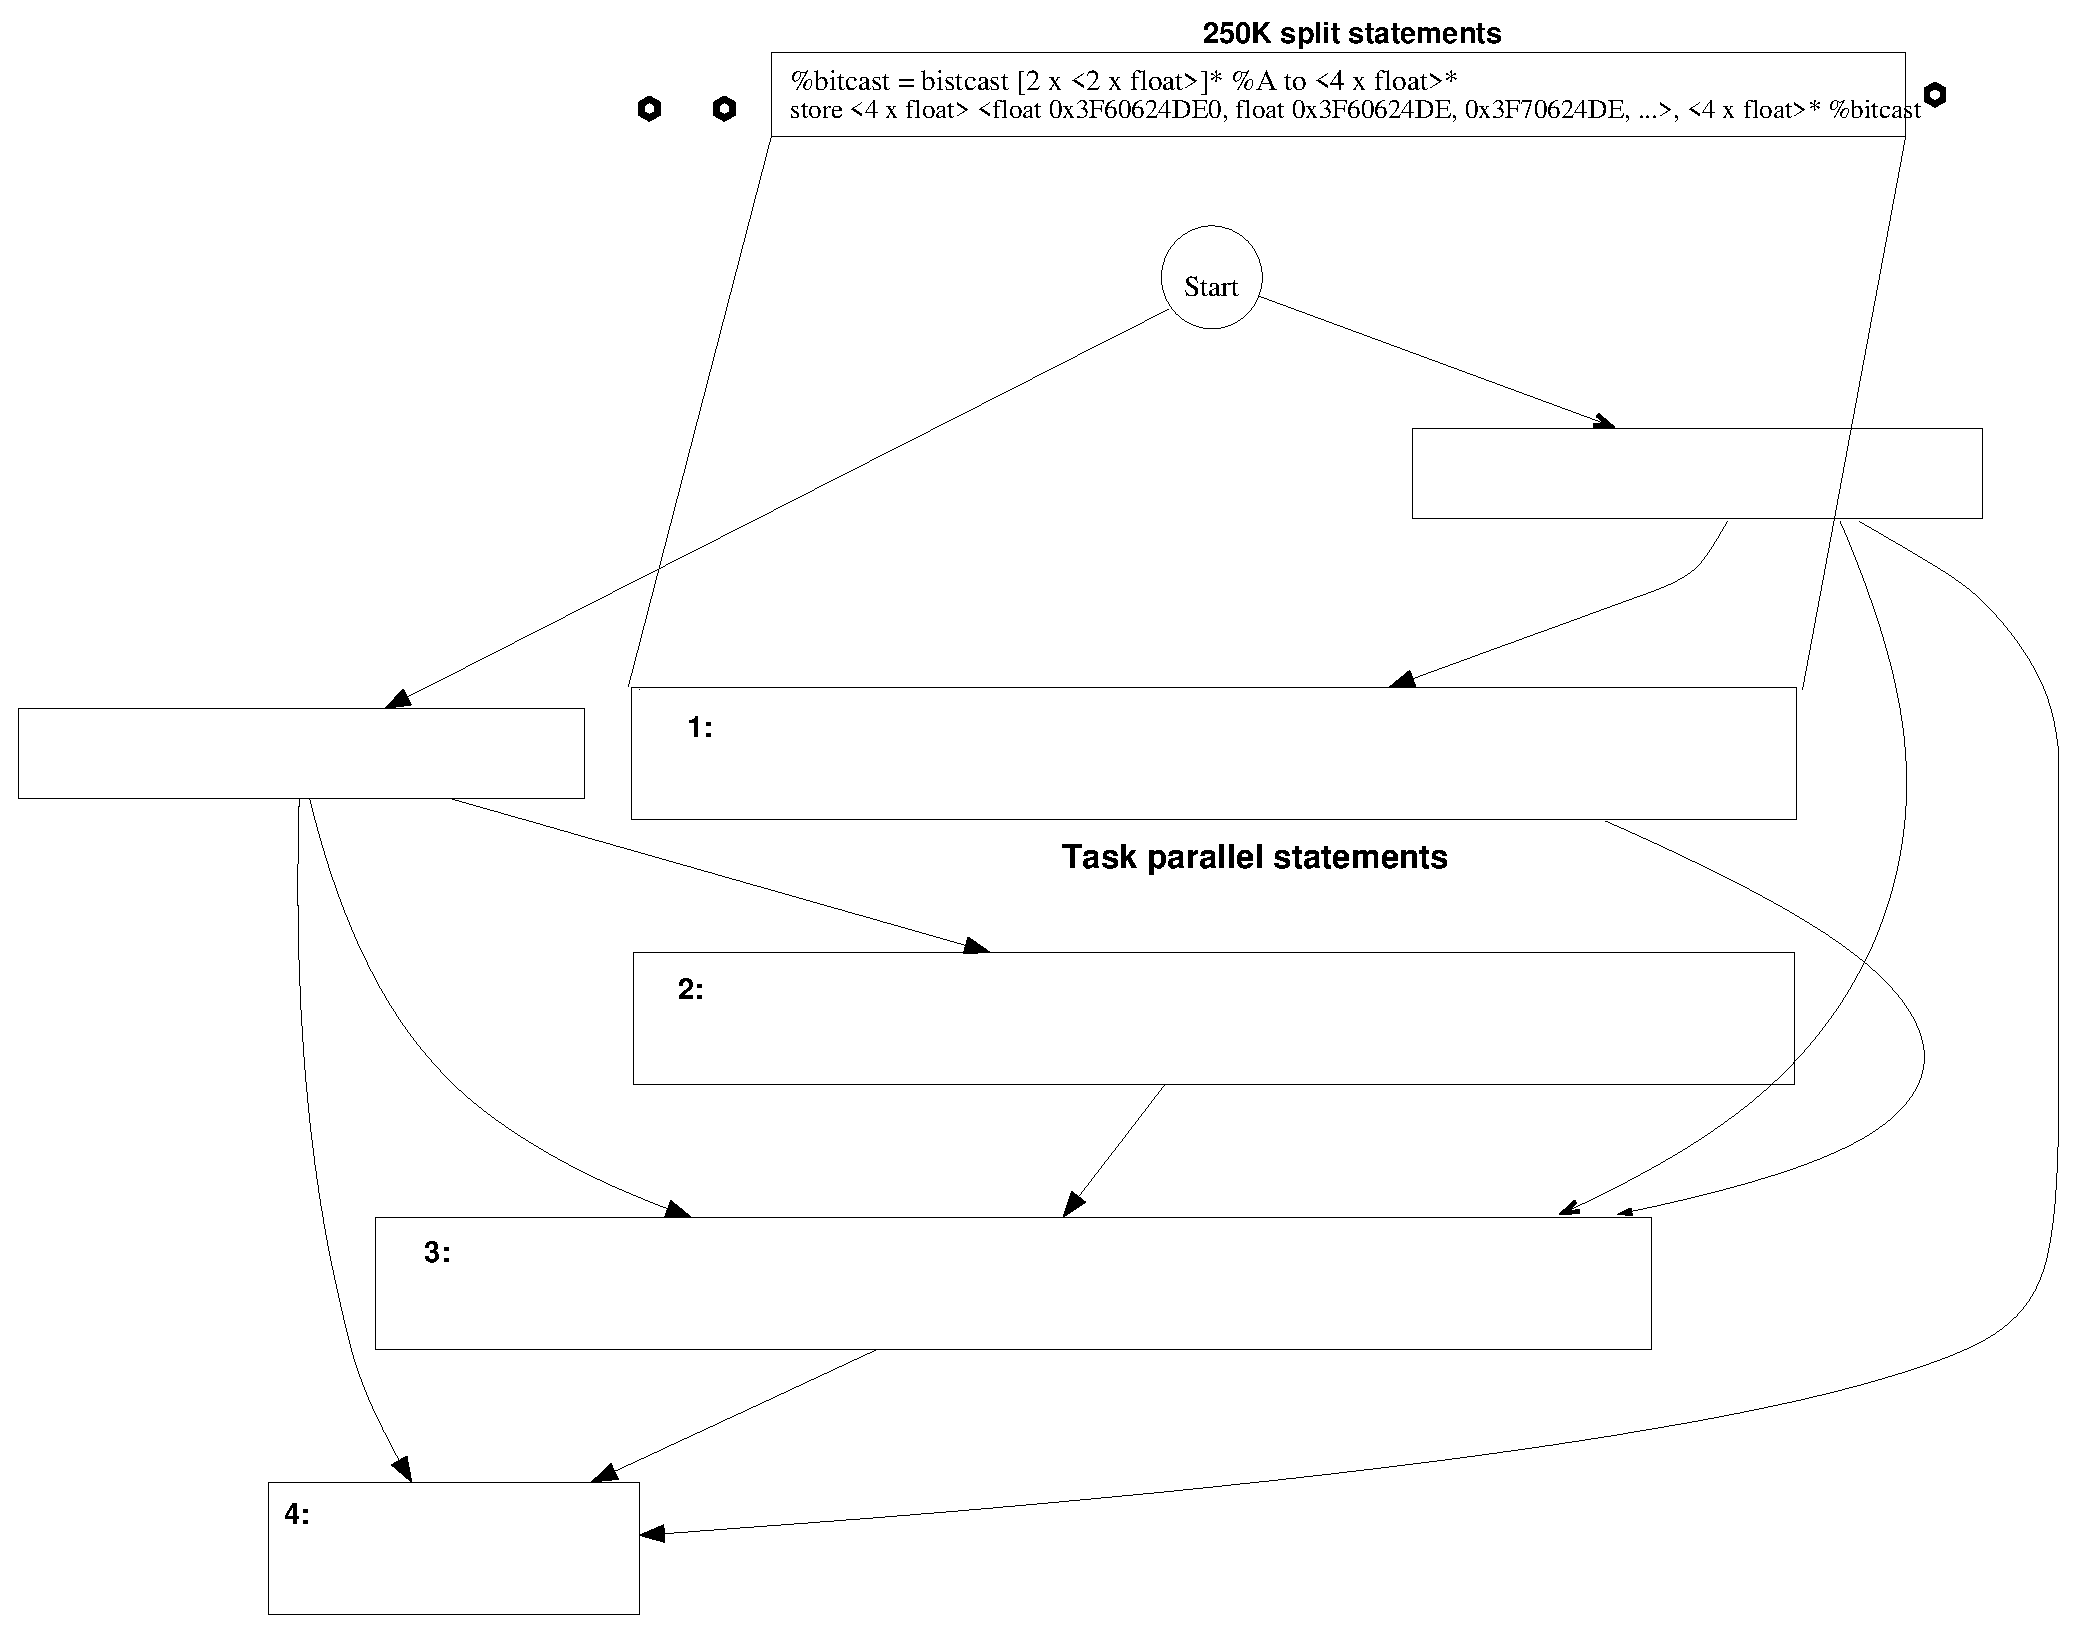
\includegraphics[scale=0.42]{./figures/jacobi2d}
  \scalebox{0.42}{\input{./figures/jacobi2d.pstex_t}}
  \caption{The task graph for the Jacobi example}
  \label{fig:1}
\end{figure*}

\begin{figure*}[t!]
  \centering
\begin{verbatim}
 % scevgep = getelementptr [1000 x <1000 x float>]* %A, i64 0, i64 %3
 % scevgep10 = bitcast <1000 x float>* %scevgep to i8*
 % uglygep = getelementptr i8* %scevgep10, i64 4
 % scevgep11 = getelementptr [1000 x <1000 x float>]* %B, i64 0, i64 %3
 % scevgep1112 = bitcast <1000 x float>* %scevgep11 to i8*
 % uglygep13 = getelementptr i8* %scevgep1112, i64 4
 call void @llvm.memcpy.p0i8.p0i8.i64(i8* %uglygep,i8* %uglygep13,i64 3996,i32 4,i1 false)
\end{verbatim}
  \caption{LLVM code for assignment statement \texttt{4} from
    Figure~\ref{fig:2}}
  \label{fig:3}
\end{figure*}

The task graph is built from the application. The compiler extracts task
and data parallelism form the application for partitioning the
application onto the architecture. The compiler looks at every statement
in the program to form the task graph. The task graph is formed in the
following manner:

\begin{itemize}

\item The assembly instruction count for every statement is obtained
  first. Currently, we look at the LLVM (Low level virtual
  machine)~\cite{clat04} instruction count. For example, the LLVM code
  generated for the assignment statement \texttt{4} in
  Figure~\ref{fig:2} is shown in Figure~\ref{fig:3}. The LLVM
  instruction count gives an approximation of the instruction count of
  the underlying hardware, while remaining independent of the hardware
  itself.

\item Every loop is fissed thereby forming multiple statements. The
  intuition behind fissing the loops is two fold: (a) task parallelism
  can be exploited by running independent loop statements separately on
  different machines (see Figure~\ref{fig:1}) and (b) the graph
  partitioner would give us feedback on the vector size of the loop,
  which can then be fused back if allocated to the same resource.

\item The vector counts for each statement is determined using
  dependence analysis and using the polyhedral model~\cite{mgri98}. The
  largest vector size requirement is given as the second constraint in
  the task graph.

\item Finally, the polyhedral model is also used to find the iteration
  count of the statements and to determine the total amount of data (in
  bits) required to process by that statement. For example, statement
  \texttt{4} (the last \texttt{boxed} statement in Figure~\ref{fig:1})
  requires \texttt{7.8085KB}, while the first two statements \texttt{1}
  and \texttt{2} require 64-bits more due to the difference in the loop
  iteration count (see Figure~\ref{fig:2}).

\item The edges in Figure~\ref{fig:1} with 0 weights are dependence
  arcs. For example, in the Jacobi example, statements \texttt{1} and
  \texttt{2} can be carried out in parallel, while statements
  \texttt{3} and \texttt{4} have a dependence on these two statements
  and hence, cannot be split.

\end{itemize}

\subsubsection{Tiling vectors}
\label{sec:tiling-vector-counts}

As we can see from Figure~\ref{fig:1}, three of the statements in Jacobi
example require almost a million vector instructions to be carried out
in parallel. The vector counts can increase quite quickly for large
examples (notice that the current 1 million vector count is just for a
1000 $\times$ 1000 Jacobi matrix). In order to properly utilize the
underlying vector hardware these vector lengths need to be split into
smaller vector lengths. The resultant vector lengths depend upon the
underlying hardware. Splitting the vector constraints is termed tiling
in the compiler community. There are many ways to tile a vector. For
example, given a single processing element with a small vector size: a
vector might be tiled to fit the underlying hardware vector size and
then run in a loop (an approach taken by the gcc compiler). If a number
of processing elements with differing vector sizes are available as is
the case of HPC architectures determining the optimal vector tiles is a
challenge and can be solved with \textit{Simulated annealing}
(SA)~\cite{tbra01} or meta \textit{Genetic algorithm} (GA)~\cite{tbra01}
heuristics. In this article we do not solve the problem of determining
the tile sizes, instead our framework allows the application designers
to plug and play with different vector tiles in-order to determine the
tile size that suits their architecture. We randomly generate different
tile sizes for experimentation.

An example tiling with 250K separate, 2 $\times$ 2 tiles for statement
\texttt{1} is shown in Figure~\ref{fig:1} with its resultant LLVM
code. It is important to mention that vectors are only single
dimensional. In Figure~\ref{fig:1}, we are type-casting a 2D matrix of
size 2 $\times$ 2 into a single dimensional 4 element vector. Such
vectorization is also called loop-collapsed vectorization, i.e., instead
of just vectorizing the inner most loop in Figure~\ref{fig:2} statement
\texttt{1}, we are collapsing the outer and inner loop into a single
vector instruction to improve performance. Such loop collapse is not
necessary and can be considered a super optimization. But, our framework
allows the application designers to explore such possibilities.



%%% Local Variables:
%%% mode: latex
%%% TeX-master: "bare_conf"
%%% End:


\subsection{Generating the resource graph}
\label{sec:gener-reso-graph}

\begin{figure*}[t!]
  \centering
  % 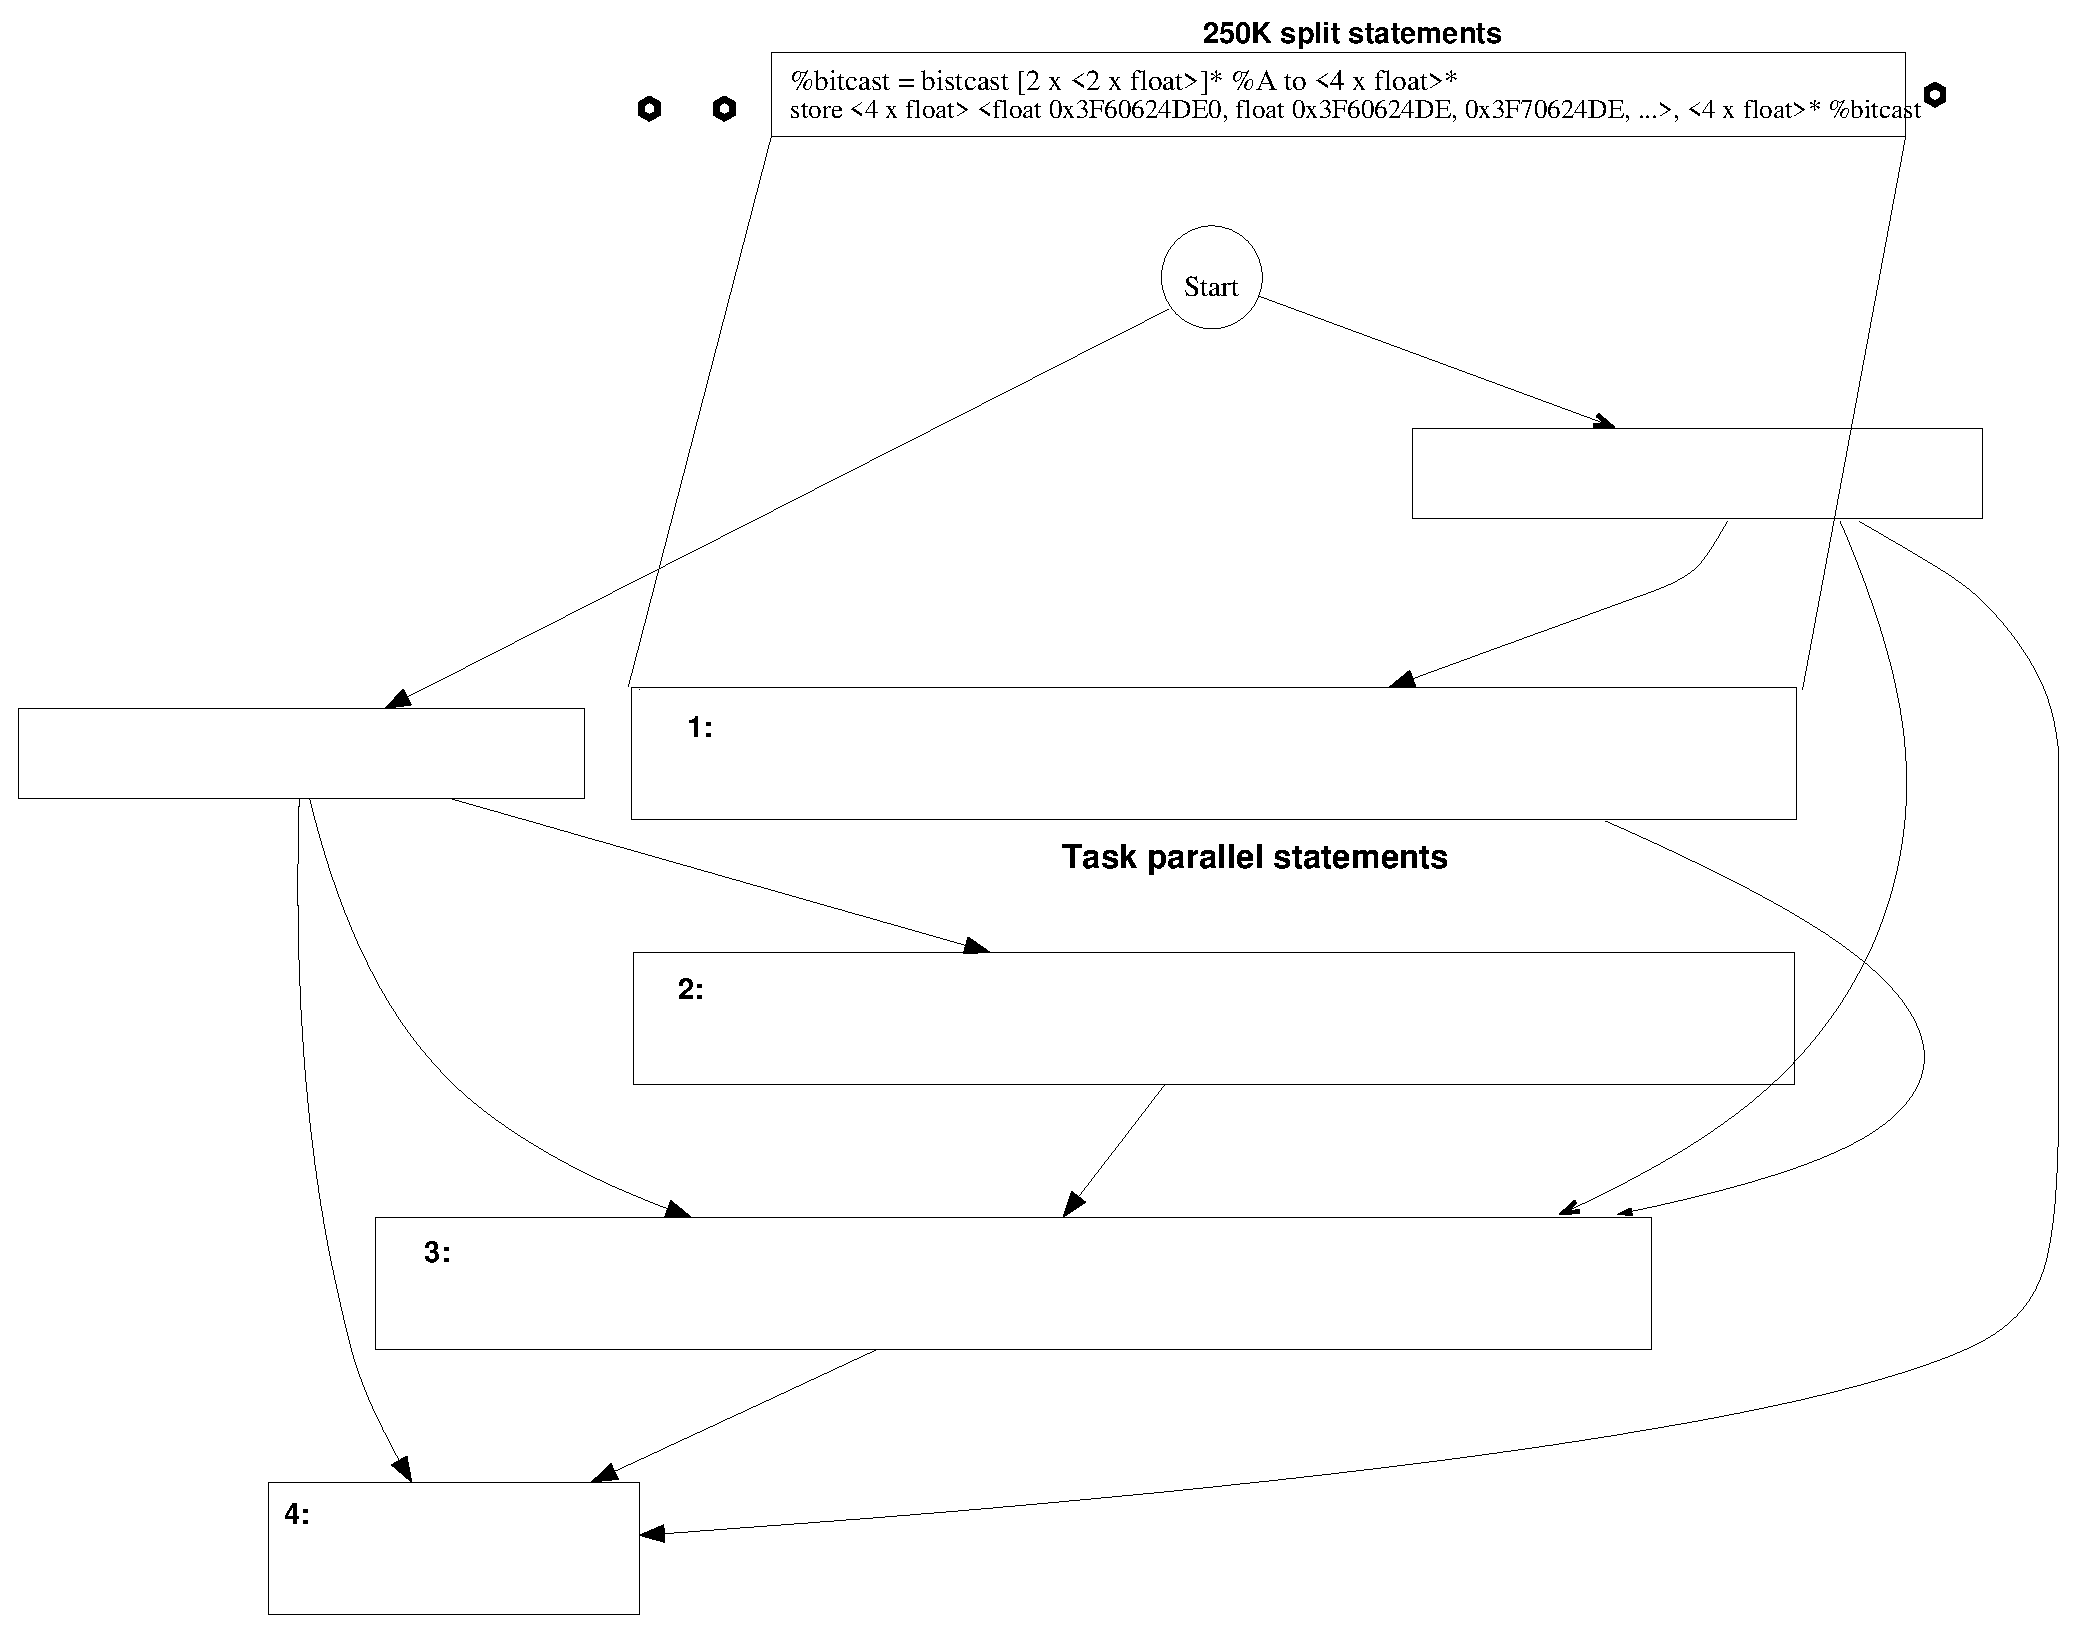
\includegraphics[scale=0.42]{./figures/jacobi2d}
  \scalebox{0.4}{\input{./figures/dendrogram.pstex_t}}
  \caption{The dendrogram for Figure~\ref{fig:res}}
  \label{fig:7}
\end{figure*}

The resource graph represents the cluster of compute nodes on which the
task graph will be executed. There are a plethora of different
architectures and topologies that an HPC architecture might be
configured in. Moreover, we cannot even predict the type of
configurations that might come up in the future. Hence, in order to
accommodate the varying types of topologies and configurations, we use
synthetic topologies to test our partitioning framework.

A sample resource graph is shown in Figure~\ref{fig:res} at level 0. The
resource graph that is shown is heterogeneous in both computation and
communication. The properties of the resource graph are described below:

\begin{itemize}

\item \textbf{Compute nodes:} The compute nodes are assumed to belong
  under two categories of processing units, mainly CPUs and
  GPUs. Following the current trend, the CPUs have a larger MIPS
  count. The MIPS capacity of a PE is denoted by the first decoration
  $R^i_0, \forall i \in V_r$. The GPU nodes have a lower MIPS count, but
  have a large resident vector length, denoted by the second decoration
  $R^i_1, \forall i \in V_r$. For example, the first PE at level 0 is a
  CPU, since it has a small vector count and a large MIPS count, the
  fifth PE on the other hand is a GPU, since the capacities are
  reversed.


  % The scalar instructions of a Processing Element (\textbf{PE}) that
  % represents a CPU is much higher that that of a GPU. At the same time
  % parallel vector operations that a \textbf{PE} representing a GPU is
  % much higher compared to that of a CPU. In Fig \ref{fig:res} $ R^1 $ is
  % a 'CPU' and $ R^5 $ is a 'GPU'.

\item \textbf{Communication links:} In the resource graph shown in
  Figure~\ref{fig:res} at level 0, follows a 2D mesh topology. In this
  topology the PEs are connected in a grid with individual communication
  links between them. The bandwidth of these links is non
  uniform. The different bandwidths on the communication links is
  represented by the decoration $E^C$.

\end{itemize}

\subsubsection{Clustering the topology}
\label{sec:clustering-topology}

Mapping the task graph on a heterogeneous architecture is a known NP
hard problem. The problem mainly lies in the size of the resouce graph
and the sheer number of ways in which the task graph can be mapped on to
the resource graph. In our approach we take a staged graph partitioning
approach. The \underline{main idea} behind our partitioning approach is
to first hierarchically cluster the nodes in the heterogeneous topology,
provided by the designer, thereby forming fewer contracted resource
nodes. The application is then partitioned in stages (levels) onto the
resulting hierarchy. The \underline{intuition} behind this approach is
two fold:

\begin{itemize}

\item \textit{Heterogeneous K-way partitioning:} If we ignore
  communication then the process of partitioning an application onto a
  given architecture is equivalent to a heterogeneous K-way partitioning
  problem. There have been successful attempts at using K-way
  partitioning for solving the partitioning problems using multiple
  different ILP formulations~\cite{fsar11}, but all have concentrated on
  a homogeneous K-way partitioning problem. Hierarchically clustering a
  heterogeneous topology such that the resulting hierarchy consists of
  contracted PEs with equivalent compute constraints can reduce the
  heterogeneous K-way partitioning problem to a homogeneous one.

\item \textit{Considering communication links:} The communication can be
  considered into the equation, while building the hierarchical cluster
  using the min-cut technique. Thus, a min-cut load-balancing of the PEs
  in a topology intuitively means: we are clustering together PEs, which
  have large bandwidth together into a single contracted node, while
  making an attempt to load balance the two constraints: MIPS and vector
  lengths.

\end{itemize}

The hierarchical cluster built for the synthetic topology at level 0 of
Figure~\ref{fig:res}, is shown in the levels 1-3. The stages used to
build the hierarchy are as follows:

\begin{itemize}

\item \textit{Effective computation during contraction:} Given a
  topology graph with $|V_r|$ resources, we cluster the PEs in levels,
  whereby the height of the cluster is $log_2|V_r|$. For example,
  consider the PEs at level 0 in Figure~\ref{fig:res}. Contraction from
  level 0 to level 1 results in 4 PEs at level 1, where the two
  capacities, $R^k_0,\ R^k_1$ for each contracted node $k = \{i, j\},
  \exists i \in V_r \wedge \exists j \in V_r$ is computed as: $R^k_0 =
  R^i_0 + R^j_0$, and $R^k_1 = R^k_1 + R^j_1$. Without loss of
  generality we assume this for any $k = \{i,j,..,n\}, \forall n \in
  V_r$. This process is continued until we reach the top-level with just
  2 contracted nodes. The resulting 2-node top-level architecture (as
  seen in Figure~\ref{fig:res}) is a load-balanced. The reason for a
  level based contraction, instead of contracting all nodes into a
  single 2 node partition, is that when partitioning the application on
  the resulting top-down cluster, we have fine grained details within
  each of the contracted node.

  % \item Firstly, we form virtual representations of the resource graph
  %   by clustering the nodes. These virtual nodes are formed by min
  %   cutting communication volume and load balancing the virtual nodes
  %   capabilities.  The formation of these virtual nodes creates
  %   homogeneous partitions from hetrogeneous PEs.

  % \item Secondly, instead of doing this in a single step, we construct
  %   this in several level by clustering half the nodes from the
  %   previous level. We end up with a structure consisting of several
  %   levels, where the $ Number\ of\ levels = log_2 ( Number\ of\ Nodes
  %   )$.

\item \textit{Effective communication during contraction:} It is
  essential that we handle communication correctly while contracting
  nodes. There are a number of paths that communication between two
  nodes might follow. The \underline{effective bandwidth} between any
  two contracted nodes depends upon the route in the topology graph
  between these contracted nodes. We use the all-pair
  Floyd-Warshall~\cite{sski08} algorithm to calculate the shortest path,
  in terms of latency of data-transfer, for every communication link
  in the topology. Once the nodes are contracted we use the bottleneck
  amongst these possible links as our effective bandwidth.

  For the topology in Figure~\ref{fig:res}, we first calculate the best
  possible paths between every pair of nodes \mbox{$(i,j) \in (V_r
    \times V_r)$}. Now let us consider the example of the contracted
  nodes \texttt{B1} and \texttt{C1}. Node $\mathtt{B1} = \{3, 8, 6\}$
  and $\mathtt{C1} = \{2, 1\}$. Being an undirected graph with loss of
  generality we can consider \texttt{B1} to be the source and
  \texttt{C1} to be the destination. Hence, the worst path, in terms of
  latency of data-transfer, following the all-pair Floyd-Warshall
  algorithm, between nodes $3$ and $2$ within the contracted nodes is
  given by the maximum latency path amongst the memoized best edges:
  $max((3,2),\ (8,2),\ (6,2))$. Similar computation is carried out for
  all link pairs in the contracted node with $1$ as the destination node
  to find the minimum latency path. Finally, the addition of these two
  latencies and its reciprocal gives us the effective bandwidth between
  the two contracted nodes. This effective bandwidth is the overall
  bottleneck between the two contracted nodes.

  % The communication bandwidth between the clustered nodes is determined
  % by,\\ ${ \sum ( \min for same destn ( \max bw R^i, R^j ) ) ) }$\\ The
  % max bandiwdths between any ${R^i}$ is determined by floyd warshall
  % algorithm.

% \item The capabity of each of the PEs that are clustered together are
% aggregated to form the larger virtual node.

% \item In each level PEs with high communication bandwidth and balanced
% capabilities are clustered together. In doing this in a bottom up
% approach i.e. clustering instead of partitioning, we allow the nodes to
% form without ignoring communication links between the nodes. This also
% avoids the formation of dangling nodes in the graph.

\end{itemize}

\begin{figure}[ht]
  % \centering
  \includegraphics[scale=0.43]{./figures/resource}
  \caption{Clustering of a resource graph}
  \label{fig:res}
\end{figure}

% In fig \ref{fig:res} we show our clustering approach on a 4x2 mesh. At
% each level suitable nodes are clustered together to form a larger node.
% We see that the PE $ R^3 $ and PE $ R^8 $ are combined together
% when moving from level 0 to level 1. Overall, we reach three levels
% and at the top most level all the nodes from a single virtual node.

\subsection{Task graph Partitioning}
\label{sec:task-graph-part}

The task partitioning on the resulting hierarchical cluster takes a
top-down approach. We start with the task-graph extracted from the
application (Figure~\ref{fig:1}). We then recursively partition the
task-graph (using K-way partitioning) on the hierarchical cluster of the
resource-graph. For the example topology cluster in
Figure~\ref{fig:res}, we start by partitioning the task-graph in
Figure~\ref{fig:1}, first into two (K=2) partitions considering two
equally weighted compute nodes at level 2. Once a partition is obtained
for this level, we move onto the next level (level 1), whereby all the
task-graph nodes allocated onto node \texttt{A2} are further partitioned
onto the nodes \texttt{A1} and \texttt{C1} (again K=2), which are
coupled into the contracted node \texttt{A2}. This process is continued
recursively for all contracted nodes until the final level (level
0). During each partition we make sure that the task node requirements
are closely matched to the resource node capacities.

% To partition the application we start with the top most level in the
% resource graph and divide it according to the required virtual nodes at
% that level. We then move on to the next level and partition the
% application on to the virtual nodes that the current node belongs to.
% In this way we follow the structure of the resource graph until we reach
% level, by which reach the actual mapping of the task graph on to the
% resource graph.

Doing it in this top down manner carries two important consequences.

\begin{itemize}

\item \textit{Increase in the time complexity:} As stated previously,
  the partitioning problem is equivalent to the K-way problem. The
  multi-level K-way partitioning results in the worst cast time
  complexity of $O(|E_t| \times log_2|V_r|)$~\cite{gkar98}. Our
  algorithm gives a worst case complexity of \mbox{$O(log_2|V_r| \times
    |E_t| \times log_2 |V_r|)$} when using the multi-level K-way
  partitioning. But, in the average case the term $log_2|V_r|$ is
  inconsequential, since we ask for a balanced 2-way partition at all
  levels. Hence, the average case complexity is equal to the K-way
  partitioning algorithm.

\item \textit{Refined mapping:} By dividing the mapping on to several
  levels we can achieve much better load balancing by considering only
  fewer nodes to map than if we were to do it directly on to the
  resource graph. We show this quantitatively in the Experimental
  results section~\ref{sec:experiments-results}.

\end{itemize}





%%% Local Variables: 
%%% mode: latex
%%% TeX-master: "bare_conf"
%%% End: 


\section{Implementation}
\label{sec:imple}

We follow a bottom up approach when clustering onto the virtual nodes
from the resource graph and top down approach when
In order to implement our heuristic we use METIS \cite{} graph
partitioning tool.

bullshit about metis.

The resource graph is generated by assuming the capabilities lie in a
fixed range. Using this we define a range from which we assign the
respective PE's capabilities. In generating them synthetically we avoid
being biased by a single architecture and we can evaluate our system
for different characteristics. The interconnect is considered to be two
dimensional mesh with varying bandwidths. Thus, making both the
computaions and communication be truly hetrogeneous.

Once we have the resource graph, we perform the clustering as describe
in section \ref{sec:gener-reso-graph}. We use metis to do the
clustering of the nodes based on communication volume min cut and load
balance constraints. The entire process is described below:

\begin{itemize}

\item The generated resource is graph is represented in the Metis
graph format. We represent the PEs capabilities as constraints of the
nodes and the link's bandiwdths as communication volume of the edges.

\item We then construct our clustered structre by halving the nodes at
each level. Metis partitions the graph by load balancing the
constraints and min cut communication. So the number of partitions
that it might provide might be less than that being requested.

\item When constructing the new virtual node, the constraints of the
previous are aggregated and the communication is calculated by summing
the minimum bandwidths of links connecting the nodes present in the
different partitions.

\item We repeat the clustering for each level, until we reach a stage
in which all the PEs form a single partition.

\end{itemize}

In partitioning the task graph, we need to balance the constraints on
to the available partitions. Metis offers the ability to load balance
multiple constraints on to different partitions based on the metric 'tp
weight'. We calculate the ratios between the capabilities of different
partitions and represent as this metric in order to load balance on to
the available partitions. The steps through which task graph follows
are,

\begin{itemize}

\item We start at the top most level in the resource graph and request
for the number of partitions equal to that of the child nodes at the
next level.

\item The capabilities of the resource graph are represented as ratios
for each of the constraint as the 'tp weight' metric when partitioning
the task graph using Metis.

\item As we go down on to each level we partition the task graph into
smaller fine grained parts until we reach the lowest level.

\item Finally, the entire task graph is partitioned into sub graphs
where each of them are mapped onto a specific PE in the resource graph.

\end{itemize}

\subsection{Load Balancing Multiple Constraints}

Metis load balances constraints by minimizing the imbalance with that
of a ideal value. It tries to acheive this by modifying the
partitioning such that each consrtaint lies within certain imbalance
from the ideal value. Since reaching a 'optimal' solution is difficult
here, it matches each of the constraint in order until it finds a
solution where all the constraints are matched within a certain
tolerance level. Unfortunately, this causes the contraint to be
matched with more and more imbalance as we move further.

In order to handle this, we chose an addition to our heuristic that
checks whether we achieve the least imbalance in compute power in our
partitions. This is done by clustering the nodes at each level based
on all the possible permutations of the resource graph. After each
clustering for a given permutation the imbalance in compute power is
calculated as,

\begin{equation}
\begin{array}{c}
desired_compute_power = total_compute_power / no_of_nodes;\\

for each partition, for 1->n\\
cp_n = sum( ( compute power of node ( R * R .. Rn ) ) -
desired_compute_power )\\

chosen partition = min( cp_n  )\\
\end{array}
\end{equation}

We then pick the partition that was yielded with the minimum deviation
in the compute power.




\section{Experiments and results}
\label{sec:experiments-results}

% To determine how good our framework is, we compare it against an
% adaptation of the well known heterogeneous bin packing solution as
% discussed by Teodor et al.~\cite{tcra11}. They adapt the well-known
% \textit{Best First Decreasing (BFD)} heuristic, which works only for
% homogeneous bins, to form the \textit{Adapted BFD (A-BFD)} heuristic
% which works for heterogeneous bins. We have chosen to compare our
% framework against a bin-packing heuristic, because it is a well known
% fact that the optimal solution for a partitioning problem is NP hard,
% one cannot find optimal solutions for large processing
% architectures. Heuristic bin packing solutions have given good results
% in the general case~\cite{ecof78}. There exists no other heuristics (to the
% best of our knowledge) other than A-BFD which is able to model both vector and
% scalar processing elements in a given architecture. Hence, comparing with
% A-BFD allows us to gauge the effectiveness of our algorithm against a standard
% technique.


\subsection{Our implementation}
\label{sec:our-implementation}

We use the Metis~\cite{gkar95} graph partitioning library to implement
our partitioning algorithm. We are not tied to Metis and any other graph
partitioner such as Zoltan~\cite{kdev09} or Scotch~\cite{cche08} can be
used for implementing our algorithm. Herein, we describe how we used
Metis to implement the graph partitioning.

The resource graph is represented in the Metis graph format. We
represent the PEs' capabilities as constraints of the nodes and the
links' bandwidths as communication weight on the edges. We then
construct our clustered structure (Figure~\ref{fig:res}) by asking for a
2-way partition at each level of the $log_2|V_r|$ height. Metis
partitions the graph by load balancing the constraints and performing a
minimum edge cut.  In partitioning the filter graph, we need to balance
the constraints on to the available partitions. Metis offers the ability
to load balance multiple constraints on to different partitions based on
the metric \mbox{`tp-weight'}. We calculate the ratios between the
capabilities of different partitions and represent them as this metric
in order to load balance on to the available partitions.


\subsection{Random Graph Generator}
\label{sec:rand-graph-generator}
We built a random graph generator to test our partitioning methodology
rigorously against a variety of application graphs. The random graph generator
needs as input the following parameters :

\begin{itemize}
\item Number of nodes ($n$) - Total number of nodes to be present in the
application graph
\item Indegree ($i$) - Average indegree of every vertex
\item Outdegree ($o$) - Average outdegree of every vertex
\item Communication to Computation Ratio - CCR ($c$) - It is the ratio
of the average communication cost of an edge leaving a vertex to the average
computation cost of the vertex the edge is leaving from. If a DAG's
$c$ is low, then it can be called a computation intensive application
and if it is greater than 1 it can be called a communication intensive
application
\item Structure of the graph ($\alpha$) - We
generate the height of the graph based on $\alpha$ as
$\frac{\sqrt{n}}{\alpha}$. This implies the width of the graph becomes
$\sqrt{n}*{\alpha}$. Higher values of $\alpha$ give wider graphs which
means the graph has more inherent parallelism, while lower values give taller
graphs which means the graph is inherently serial
\item Beta ($\beta$) - We use this parameter to decide if an actor in the
application graph is CPU intensive or GPU intensive. Smaller values of $\beta$
makes actors CPU intensive(by making first constraint larger than the second),
while larger values make it GPU intensive(bu making the second constraint larger
than the first)
\item Skewedness factor ($\gamma$) - This parameter dictates how computation is
spread across the graph. Smaller values of $\gamma$ give uniformly distributed
values for the constraints of the actors while larger values produces skewed
graphs
\end{itemize}

For our experiments we generated random graphs by choosing values for the input
parameters from the following sets :

\begin{itemize}
\item $\chi_{n} = \{256, 1024, 16384\}$
\item $\chi_{i} = \{1\}$
\item $\chi_{o} = \{2, 4, 8\}$
\item $\chi_{c} = \{0.0001, 0.001, 0.009\}$
\item $\chi_{\alpha} = \{0.1, 1.0, 10.0\}$
\item $\chi_{\beta} = \{5, 25, 50, 75, 95\}$
\item $\chi_{\gamma} = \{25, 50, 75\}$
\end{itemize}

We generated one graph per combination for a total of [servesh fill this number
in]. Since the random graph generator has a variety of inputs and these inputs
are filled in from a large set of possible values, a diverse set of DAGs are
generated with various characteristics. Experiments based on diverse set of DAGs
prevent biasing towards a particular partitioning algorithm.

% \subsection{Heterogeneous Bin Packing}

% Let $\mathcal{I}$ be the items to be accommodated into the bins and let
% $\mathcal{K}$ be the set of bins available.  From the standpoint of the
% mapping problem, $\mathcal{I}$ refers to the set of
% \mbox{application-filters ($|V_t|$)} and $\mathcal{K}$ refers to the PEs
% ($|V_r|$). Similar to the Knapsack problem~\cite{sski08}, by which A-BFD
% is inspired, each element $i \in \mathcal{I},\ \mathcal{K}$ has two
% constraints on them represented by \mbox{$c_i$ (cost)}, which models
% $R^i_0$ and $V_i$ (volume), which models $R^i_1$, capabilities of the
% resource graph, respectively.

% \textit{A-BFD} proceeds to sort $\mathcal{I}$ according to
% non-increasing order of their volume and sorts $\mathcal{K}$ according
% to non-increasing order of the ratio $c_i/V_i$. Then, it proceeds to
% allocate items from $\mathcal{I}$ into best bins $b \in \mathcal{S}$. A
% ``best" bin, i.e., the bin with maximum free space, is defined as the
% bin volume minus the sum of volumes of the items loaded into
% it.

% The post pass in \textit{A-BFD} chooses every bin that has atleast one
% item allocated to it and tries to find an empty bin, that has a higher
% or equal volume than the allocated volume on the chosen bin but also has
% a lower cost. If it finds such an empty bin, then it transfers all the
% items allocated to the chosen bin to the newly found empty bin which is
% cheaper. One of the main advantages of\ \textit{A-BFD} is that it is
% very fast with a best case complexity of $O(N_\mathcal{I})$ without the
% post pass, where $N_\mathcal{I}$ is the number of items (number of filters
% $|V_t|$ in the filter graph $G_t$). Including the post pass, the best case
% complexity becomes $O(N_\mathcal{I} + N_\mathcal{K})$ where
% $N_\mathcal{K}$ is the number of bins (number of PEs $|V_r|$ in the
% resource graph $G_r$).

\subsection{The experimental set-up}
\label{sec:experimental-setup}

The experimental set-up consists of the resource graph generation and the
filter graph generation. Herein, we describe the two set-ups.

\subsubsection{The resource graph set-up}
\label{sec:resource-graph-setup}

The experimental set up consists of the following.

\begin{enumerate}

\item An interconnection network with \numtplgynodes
  nodes. \numtplgynodes vary from 64 to 4096 PEs. A node can be just a
  multi-core CPU or a multi-core CPU with an attached GPU.

\item A set of \gpunum GPUs where \gpunum is at most \numtplgynodes. The
  GPUs are connected in the network at locations, chosen randomly in the
  normal distribution of 25\% to 75\% of $|V_r|$.

\item A set $\veclenset = \{G_1, G_2, G_3, ... G_{|\veclenset|}\}$ where
  $G_i$ is a power of 2.  Every GPU in this experiment has a vector
  length of $G_i$ where $G_i$ is sampled randomly from the set
  \veclenset. The elements of set \veclenset are chosen from a normal
  distribution ranging from: 1024 to 16284.

\item A set $\corenumset = \{C_1, C_2, C_3, ... C_{|\corenumset|}\}$
  where $C_i$ is a power of 2.  Every CPU in this experiment has $C_i$
  cores where $C_i$ is sampled randomly from the set \corenumset.

\item A set $\mipsset = \{M_1, M_2, M_3, ... M_{|\mipsset|}\}$ where
  $M_i$ is a power of 2.  Every $C_i \in \corenumset$ and GPU in this
  experiment has a MIPS count of $M_i$ where $M_i$ is sampled randomly
  from the set \mipsset. The elements of set \mipsset are chosen from a
  normal distribution ranging from: XXX to XXX.

\end{enumerate}

For given values of \numtplgynodes, \gpunum, \veclenset, \corenumset,
and \mipsset and a given application, let the $k$-th \ul{trial} be
defined as one execution of the following sequence of steps.

\begin{itemize}

\item For each GPU $G_i$, sample \veclenset and \mipsset randomly to
  determine its vector length $V_i$ and MIPS count $M_i$. \label{i1}

\item For each CPU $P_i$, sample \corenumset randomly to determine the
  number of cores $C_i$ in the processor $P_i$.~\label{i2}

\item For each core $C_i$ in the processor $P_i$ sample $V_i$ and $M_i$
  randomly from set \veclenset and \mipsset.

\item Use our framework to extract data and filter parallelism that is
  best utilizable by the heterogeneity created by parameters in items 1,
  2, and 3 above. Determine the execution time
  $L^{\mathcal{M}}$.

\end{itemize}

An experiment, \expt(\numtplgynodes, \gpunum, \veclenset, \corenumset
\mipsset), consists of conducting enough of the above trials so that
width of the 95\% confidence interval on the average value of
$Latency^{\zeta_\mathcal{M}}$ is less than 10\% of the average
value. This results in a variable number of trials with different
experimental set-ups. Note that two trials differ from each other only in
the seed for the random number generator.  This reduces the dependence
of our results on a lucky sequence of numbers from the random number
generator.

\subsubsection{Random filter graph generation}
\label{sec:filter-graph-setup}

% We chose 5 applications from the HPC arena: binomial option pricing (a
% financial derivatives application), 2-dimensional convolution (for image
% processing), Gram Schmidt linear algebra kernel, 2-dimensional
% Gauss-Seidel stencil computations, and finally our motivating example
% itself the 2-dimensional Jacobi stencil computation. Next for these 5
% applications, we varied the vector strip from 10 to 50, which resulted
% in graphs varying from around 50 to 5000 nodes and with 23 to 12,000
% edges. For example, given a filter node with a vector length requirement
% ($T^i_1$) of 30,000 elements, a vector strip of 10 means dividing the
% total vector requirement by 10, which results in 10 nodes each requiring
% 3000 vector elements. Similarly, the LLVM instruction count ($T^i_0$)
% for each node varies depending upon the application at hand.

% A detailed description of the applications and their features is shown
% in Table~\ref{tab:1}. In general the vector requirement of the
% applications in our benchmark suite varies from 1000 to 1 Million
% elements. The LLVM instruction count varies from around 1 to 0.3
% billion. The edge weights depicting the amount of data transfer on the
% other hand varies from 3000 bytes to almost 4.8 Mega byte.

% \begin{small}
%   \begin{table}[h!]
%     \centering
%     \resizebox{!}{38mm}{
%       \begin{tabular}{|c|c|c|c|}
%         \hline
%         \textbf{Application} & \textbf{Vector strip} & $|V_t|$ & $|E_t|$ \\
%         \hline
%         \multirow{5}{*}{Binomial option pricing} & 10 & 82 & 206 \\
%         & 20 & 102 & 306 \\
%         & 30 & 122 & 406 \\
%         & 40 & 142 & 506 \\
%         & 50 & 162 & 606 \\
%         \hline
%         \multirow{5}{*}{Convolution} & 10 & 79 & 143 \\
%         & 20 & 89 & 173 \\
%         & 30 & 99 & 203 \\
%         & 40 & 109 & 233 \\
%         & 50 & 119 & 263 \\
%         \hline
%         \multirow{5}{*}{Gram Schmidt} & 10 & 228 & 443 \\
%         & 20 & 838 & 1653 \\
%         & 30 & 1848 & 3663 \\
%         & 40 & 3258 & 6473 \\
%         & 50 & 5068 & 10083\\
%         \hline
%         \multirow{5}{*}{Gauss-Seidel} & 10 & 227 & 531 \\
%         & 20 & 837 & 2041 \\
%         & 30 & 1847 & 4551 \\
%         & 40 & 3257 & 8061 \\
%         & 50 & 5067 & 12571\\
%         \hline
%         \multirow{5}{*}{Jacobi} & 10 & 48 & 130 \\
%         & 20 & 78 & 240 \\
%         & 30 & 108 & 350 \\
%         & 40 & 138 & 460 \\
%         & 50 & 168 & 570\\
%         \hline
%       \end{tabular}
%     }
%     \caption{The filter graph set-up}
%     \label{tab:1}
%   \end{table}
% \end{small}

% % We have done experiments for several different sets of parameters. In
% % this paper we show the results for the parameters enumerated in Table
% % \ref{parametr_tbl}.

% \begin{figure*}[t!]
%   \centering
%   \subfigure[Binomial Option Pricing]{
%     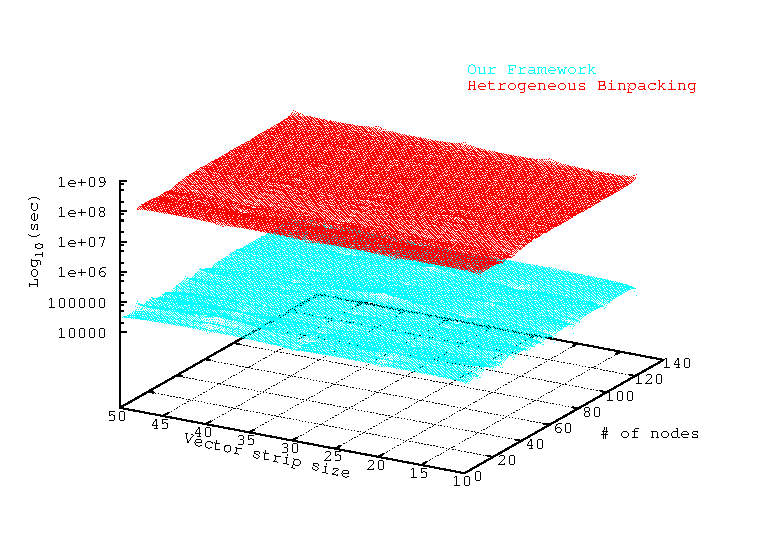
\includegraphics[angle=0, scale=0.7]{./figures/bin_surface}
%     \label{fig:bin1ho}
%   }
%   \subfigure[2 Dimensional Convolution]{
%     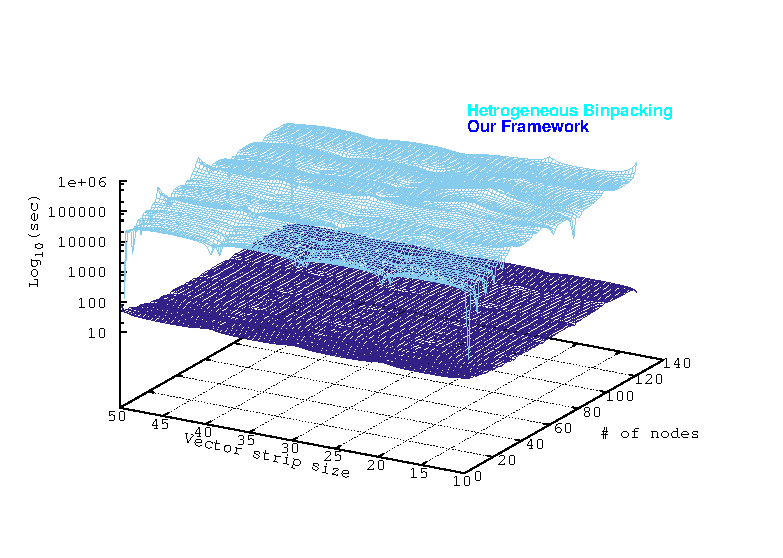
\includegraphics[angle=0, scale=0.7]{./figures/conv_surface}
%     \label{fig:conv1ho}
%   }
%   \subfigure[Gram Schmidt linear-algebra kernel]{
%     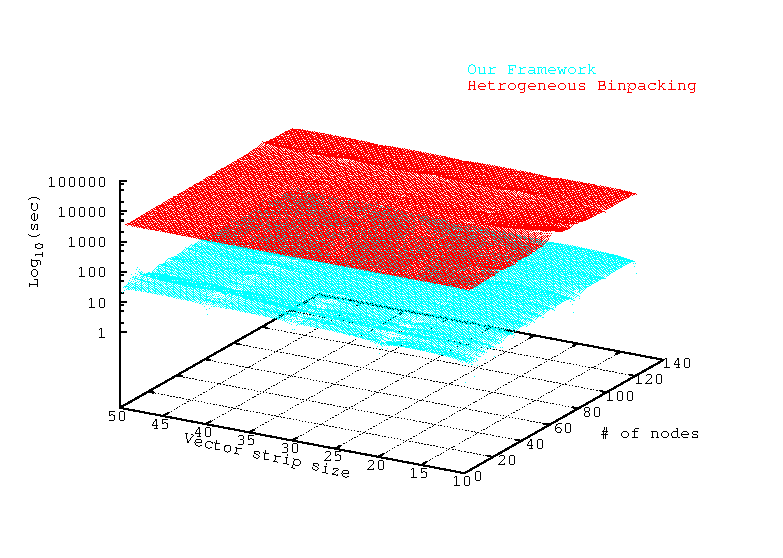
\includegraphics[angle=0, scale=0.7]{./figures/gram_surface}
%     \label{fig:gram1ho}
%   }
%   %~ \subfigure[2 Dimensional Seidel stencil computation]{
%     %~ 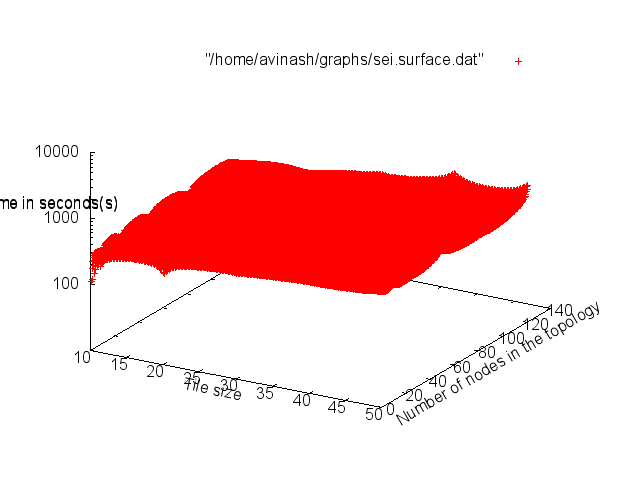
\includegraphics[angle=0, scale=0.72]{./figures/sei_surface}
%     %~ \label{fig:sei1ho}
%   %~ }
%   \subfigure[2 Dimensional Jacobi stencil computation]{
%     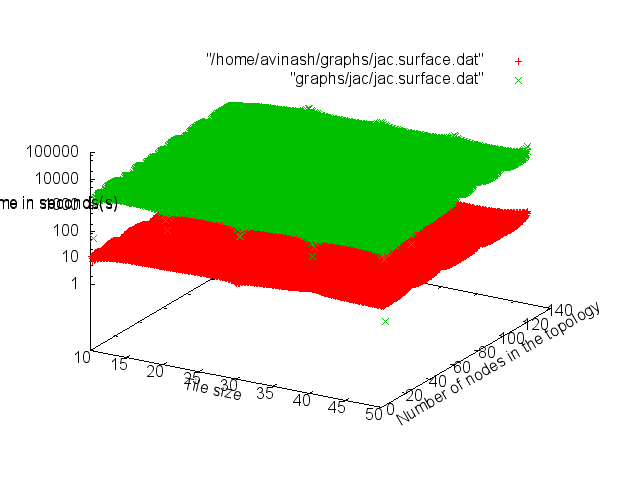
\includegraphics[angle=0, scale=0.7]{./figures/jac_surface}
%     \label{fig:jacl1ho}
%   }
%   \caption{Comparison of execution times of ``Our Framework" and
%     ``Heterogeneous Bin Packing"}
%   \label{fig:ho}
% \end{figure*}

% \begin{figure*}[t!]
%   \centering
%   \subfigure[Binomial Option Pricing]{
%     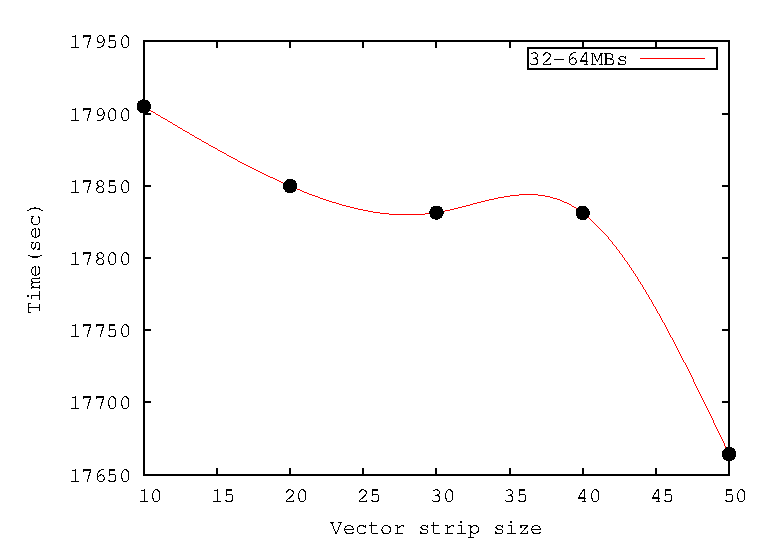
\includegraphics[angle=0, scale=0.55]{./figures/bin_32-64_surface}
%     \label{fig:bin1comm}
%   }
%   \subfigure[2 Dimensional Jacobi stencil computation]{
%     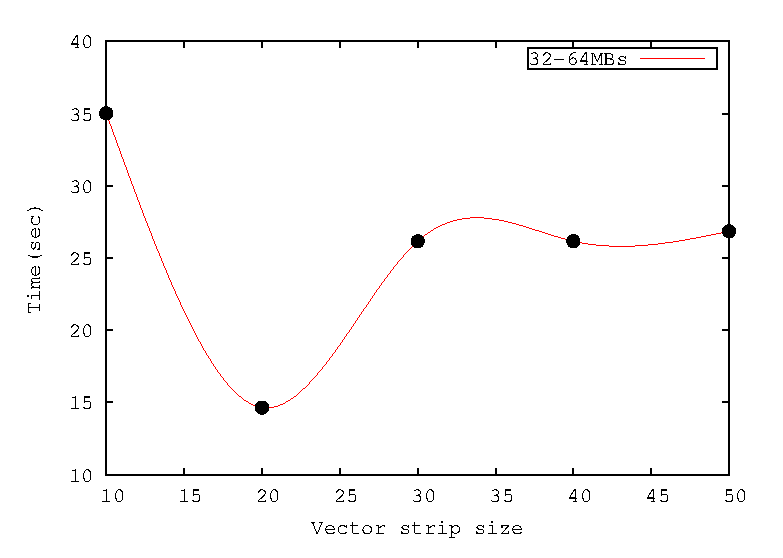
\includegraphics[angle=0, scale=0.55]{./figures/jac_32-64_surface}
%     \label{fig:jac1comm}
%   }
%   \caption{Choosing the proper tile size}
%   \label{fig:comm}
% \end{figure*}

\subsection{Experimental Results}
\label{sec:results-1}

The experimental set-up consists of a dual socket system consisting of
Intel Xeon E5620 CPU running at 2.4Ghz with 24GB DDR3 RAM. The system
is running Linux kernel ver 3.0.40-1. Our framework was compiled
using gcc version 4.7.1 with '-O3' optimization flag.

% The results for the experiments with the above experimental set-up
% comparing our approach with the aforementioned heterogeneous bin packing
% approach is shown in Figure~\ref{fig:ho}. Our approach performs better
% compared to heterogeneous bin packing for all the applications. The
% graphs in Figure~\ref{fig:ho} consists of two surfaces layered on top of
% each other. In these graphs the larger the value, the worse the latency
% and hence the performance of the application. % For all graphs, the
% % surface representing the heterogeneous bin-packing solution is always
% % layered atop our results, which clearly show the superiority of our
% % approach. Note that the z-axis in all the graph in Figure~\ref{fig:ho}
% % are in logarithmic scale with a base of 10. This in turn implies that
% % our results are almost an order of magnitude better than those
% % obtained by the heterogeneous bin packing heuristic.

% For Seidel, the results for bin-packing could not be obtained, because
% the required vector element length was larger than the available
% capability of the underlying hardware. Our approach is able to deal with
% such a situation, by fitting the required vector length to the
% capability and then running the rest in an iterative manner.

% The major differences between the two algorithms are provided in
% Table~\ref{tab:2}. The \textbf{Max latency} and \textbf{Min latency}
% columns give the maximum and the minimum latencies for bin packing and
% our framework, respectively. The final column gives the number of data
% points that our framework is better compared to heterogeneous bin
% packing. As we can see from Table~\ref{tab:2}, our framework out
% performs the heterogeneous bin-packing on all the applications.

% \begin{small}
%   \begin{table*}[t!]
%     \centering
%     \resizebox{!}{11mm}{
%       \begin{tabular}{|c|c|c|c|c|c|}
%         \hline
%         \textbf{Application} &
%         \multicolumn{2}{|c|}{\textbf{Max latency (sec)}} &
%         \multicolumn{2}{|c|}{\textbf{Min latency (sec)}} &
%         \textbf{Better (\%)} \\
%         \hline
%         & {HBP} & {Our framework} &
%         {HBP} & {Our framework} & HBP vs Our framework\\
%         \hline
%         Binomial option pricing & $1.35e+8$ & $5.27e+7$ & 77356.9 & 1 & 100 \\
%         \hline
%         Convolution & 489065 & 78.52 & 53.64 & 16.26 & 94\\
%         \hline
%         Gram Schmidt & 18984.5 & 177.97 & 2947.65 & 1.20 & 94\\
%         \hline
%         Gauss-Seidel & N/A & 3635.62 & N/A & 9.67 & 100\\
%         \hline
%         Jacobi & 13919.2 & 39.89 & 1.69 & 0.97 & 92\\
%         \hline
%       \end{tabular}
%     }
%     \caption{Major statistics comparing heterogeneous bin packing and our framework}
%     \label{tab:2}
%   \end{table*}
% \end{small}

% There are a number of reasons for the large differences seen in
% Figure~\ref{fig:ho}.

% \begin{itemize}

% \item The bin packing solution gives priority to volume, which means
%   vectors are packed into a single large vector processor, while giving
%   very little consideration to the instruction count requirement.

% \item The bin packing heuristic does not consider placing data-stores in
%   the correct locations, in fact data-stores do not play a part in the
%   whole process at all and the same can be said about communication.

% \item Bin-packing ignores communication unlike our framework.

% \end{itemize}

% In order to show how communication can have a significant
% effect on the application design and parallelism potential, in the next
% section we perform design space exploration with the effect
% of communication as the main objective.

%~ Since communication does not play a part in the heuristic bin-packing
%~ solution, we ignored the communication values when comparing with bin
%~ packing. However, in order to show how communication can have a significant
%~ effect onto the application design and parallelism potential, in the next
%~ section we perform design space exploration with the effect
%~ of communication as the main objective.

% \subsection{Affects of varying communication}
% \label{sec:arch-expl-with}

% % In the previous section we compared our results with heterogeneous bin
% % packing, without any regards for the communication. This was done by
% % keeping the bandwidth of the resource graph links high enough to not
% % have any affect on the overall application latency. We purposely did
% % this, in order to make a fair comparison with bin packing since it does
% % not consider communication when partitioning the nodes in the filter
% % graph.

% In this section we vary the bandwidth (weights on the resource graph
% edges, $E^C$) to explore best vector tile sizes for the applications.
% For experimental purposes, we use a 2D tiled mesh of 16 $\times$ 16 PEs
% (total of 256 PEs). The bandwidth of the links is randomly selected from
% a normal distribution between 32-64 MB/s for each edge. In this set-up,
% a GPU-CPU combination is placed at every fourth corner in the tiled
% mesh. Finally, every CPU core in this set-up runs at 2GHz and has a
% vector capacity of 64, i.e., 64 floating point elements can be processed
% at once. Similarly, all GPUs run at 700MHz and can perform 4096 floating
% point operations in a SIMD fashion. The application set is varied in the
% exact same manner as the previous experimental set-up.


% Two of the most interesting results that we obtained for the above
% experimental set-up is shown in
% Figure~\ref{fig:comm}. Figure~\ref{fig:bin1comm}, gives the varying
% latency of execution for the different vector strip sizes for the
% binomial option pricing application. As we can see, with increasing
% vector strip sizes the latency of execution reduces. In our experiments
% we found that a vector strip size of 50 is best suited for this example
% and gave the best performance. Moreover, we also found that from the 256
% PEs, this example only utilized 46 PEs and that too mostly GPUs.  Jacobi
% on the other hand performs best for a vector strip size of
% 20. Increasing the vector strip size after that has an adverse affect on
% the resulting partitioning as the communication overheads are far
% greater than the computation potential. Finally, in both these
% applications the placement of the data stores plays an important role,
% since there is a single data store, which needs to be accessed by all
% the nodes split due to vector tiling, the communication overhead
% increases if the store is not placed on a correct PE: usually a PE with
% high bandwidth connection to the PE processing the vector statement.

%%% Local Variables:
%%% mode: latex
%%% TeX-master: "bare_conf"
%%% End:


\section{Conclusion}
\label{sec:conclusion}

The conclusion goes here. this is more of the conclusion

% use section* for acknowledgment
% \section*{Acknowledgment}


% The authors would like to thank...
% more thanks here


% trigger a \newpage just before the given reference
% number - used to balance the columns on the last page
% adjust value as needed - may need to be readjusted if
% the document is modified later
%\IEEEtriggeratref{8}
% The "triggered" command can be changed if desired:
%\IEEEtriggercmd{\enlargethispage{-5in}}

% references section

% can use a bibliography generated by BibTeX as a .bbl file
% BibTeX documentation can be easily obtained at:
% http://www.ctan.org/tex-archive/biblio/bibtex/contrib/doc/
% The IEEEtran BibTeX style support page is at:
% http://www.michaelshell.org/tex/ieeetran/bibtex/
%\bibliographystyle{IEEEtran}
% argument is your BibTeX string definitions and bibliography database(s)
%\bibliography{IEEEabrv,../bib/paper}
%
% <OR> manually copy in the resultant .bbl file
% set second argument of \begin to the number of references
% (used to reserve space for the reference number labels box)

\scriptsize{
\bibliographystyle{IEEEtran}
% \bibliography{latex8}
\bibliography{/Users/amal029/Dropbox/BIBLIOGRAPHY_DATABASE/main_bib.bib}
}

% that's all folks
\end{document}



%%% Local Variables: 
%%% mode: latex
%%% TeX-master: t
%%% End: 
